\documentclass{article}
\usepackage{amsmath}
\usepackage{amsthm}
\usepackage{amsfonts}
\usepackage{amssymb}
\usepackage{bbold}
\usepackage{dsfont}
\usepackage{graphicx}
\usepackage{cleveref}
\usepackage{bm}
\usepackage{booktabs}
\usepackage{siunitx}
\usepackage{xcolor}
\usepackage{pdfpages}
\usepackage[utf8]{inputenc}
\usepackage[english]{babel}
\newtheorem{definition}{Definition}
\newtheorem{example}{Example}
\newcommand{\exP}[1]{\mathrm{e}^{#1}}
\newcommand{\dif}{\mathrm{d}}
\renewcommand{\vec}[1]{\mathbf{#1}}
\newcommand{\pdagger}{{\phantom{\dagger}}}
\newcommand{\state}[1]{\vert #1\rangle}
\newcommand{\cstate}[1]{\langle #1\vert}
\newcommand{\tr}[1]{\mathrm{tr}\left\{#1\right\}}
\newcommand{\trs}[2]{\, \mathrm{tr}_{#1}\{#2\}}
\newcommand{\expc}[3]{\langle #1\vert #2 \vert #3\rangle}
\usepackage[doi=false,url=false,isbn=false,backend=bibtex,style=nature,natbib=true,sorting=none]{biblatex}
\bibliography{bib.bib}
\usepackage{geometry}
\geometry{
	a4paper,
	total={170mm,257mm},
	left=15mm,
	right=15mm,
	top=15mm,
}
\begin{document}
\title{Report 24}
\maketitle

Questions/requests:
\begin{itemize}
	\item Convergence: How does increasing the number of trajectories change currents and spin selectivity? 
	\item Limit cycles/steady states: Do individual trajectories, for the cases, in which the currents oscillate at long times, go to a limit cycle? If yes, is there a single or multiple limit cycles? 
	\item Compare different ways to obtain spin selectivity/analyse the data: 
	\begin{itemize}
		\item Ensemble-average $I_+$ and $I_-$, take time-average, compute $S$ from these time averages.
		\item Time-average $I_+$ and $I_-$ over period $T$ of oscillation for each trajectory independently, compute $S$.
		\item Fourier-analysis of currents. 
	\end{itemize}
\end{itemize}

Short summary of findings:
\begin{itemize}
	\item Analysis of ensemble-average of time-averaged currents for a varying number of trajectories (figs. 6, 7) shows a very slow convergence of the ensemble average to the mean. The computed distribution of time-averaged currents does not follow a normal distribution as there is a significant number of outliers. 
	A spin selectivity can be obtained from the averaged currents. This quantity, however, also suffers from poor convergence with number of trajectories. 
%	The poor convergence to the mean and the distribution of currents indicate that at least the first moment of the analytical distribution function of the current is not well-defined. What if the distribution is simply multimodal, as one expect from a potential energy surface with multiple minima?
	\item In smaller systems ($L\leq 5$ sites), limit cycles or stationary states of the individual trajectories can be identified from the quasi-periodicity of the system energy at long times. In all investigated systems, there are multi-stabilities which lead to very different limit cycles (the observables also might be very different).  
	\item Systems with larger than $L>5$ sites, no (quasi-)periodicity of the trajectories can be identified on the time-scale investigated so far. 
	\item The problem with obtaining spin selectivities for each trajectory is that they might not be well-defined when currents cross the zero. From a practical point of view it is not clear how determine the initial and final time points for many trajectories, since not all trajectories lead to (quasi-)periodically oscillating currents.    
\end{itemize}
\clearpage
\section{Convergence with number of trajectories}
In the following, Franssons model with $L=1\times 5$ is considered.
The plots in \cref{fig:1_E_I_S} shows energy of the molecule, currents for lead polarization $P=0.5$ (majority spin "up" in the left lead), and spin selectivity, averaged over an ensemble of 31 trajectories (blue lines) and 401 trajectories (black lines).
\begin{figure}[!h]
	\centering
	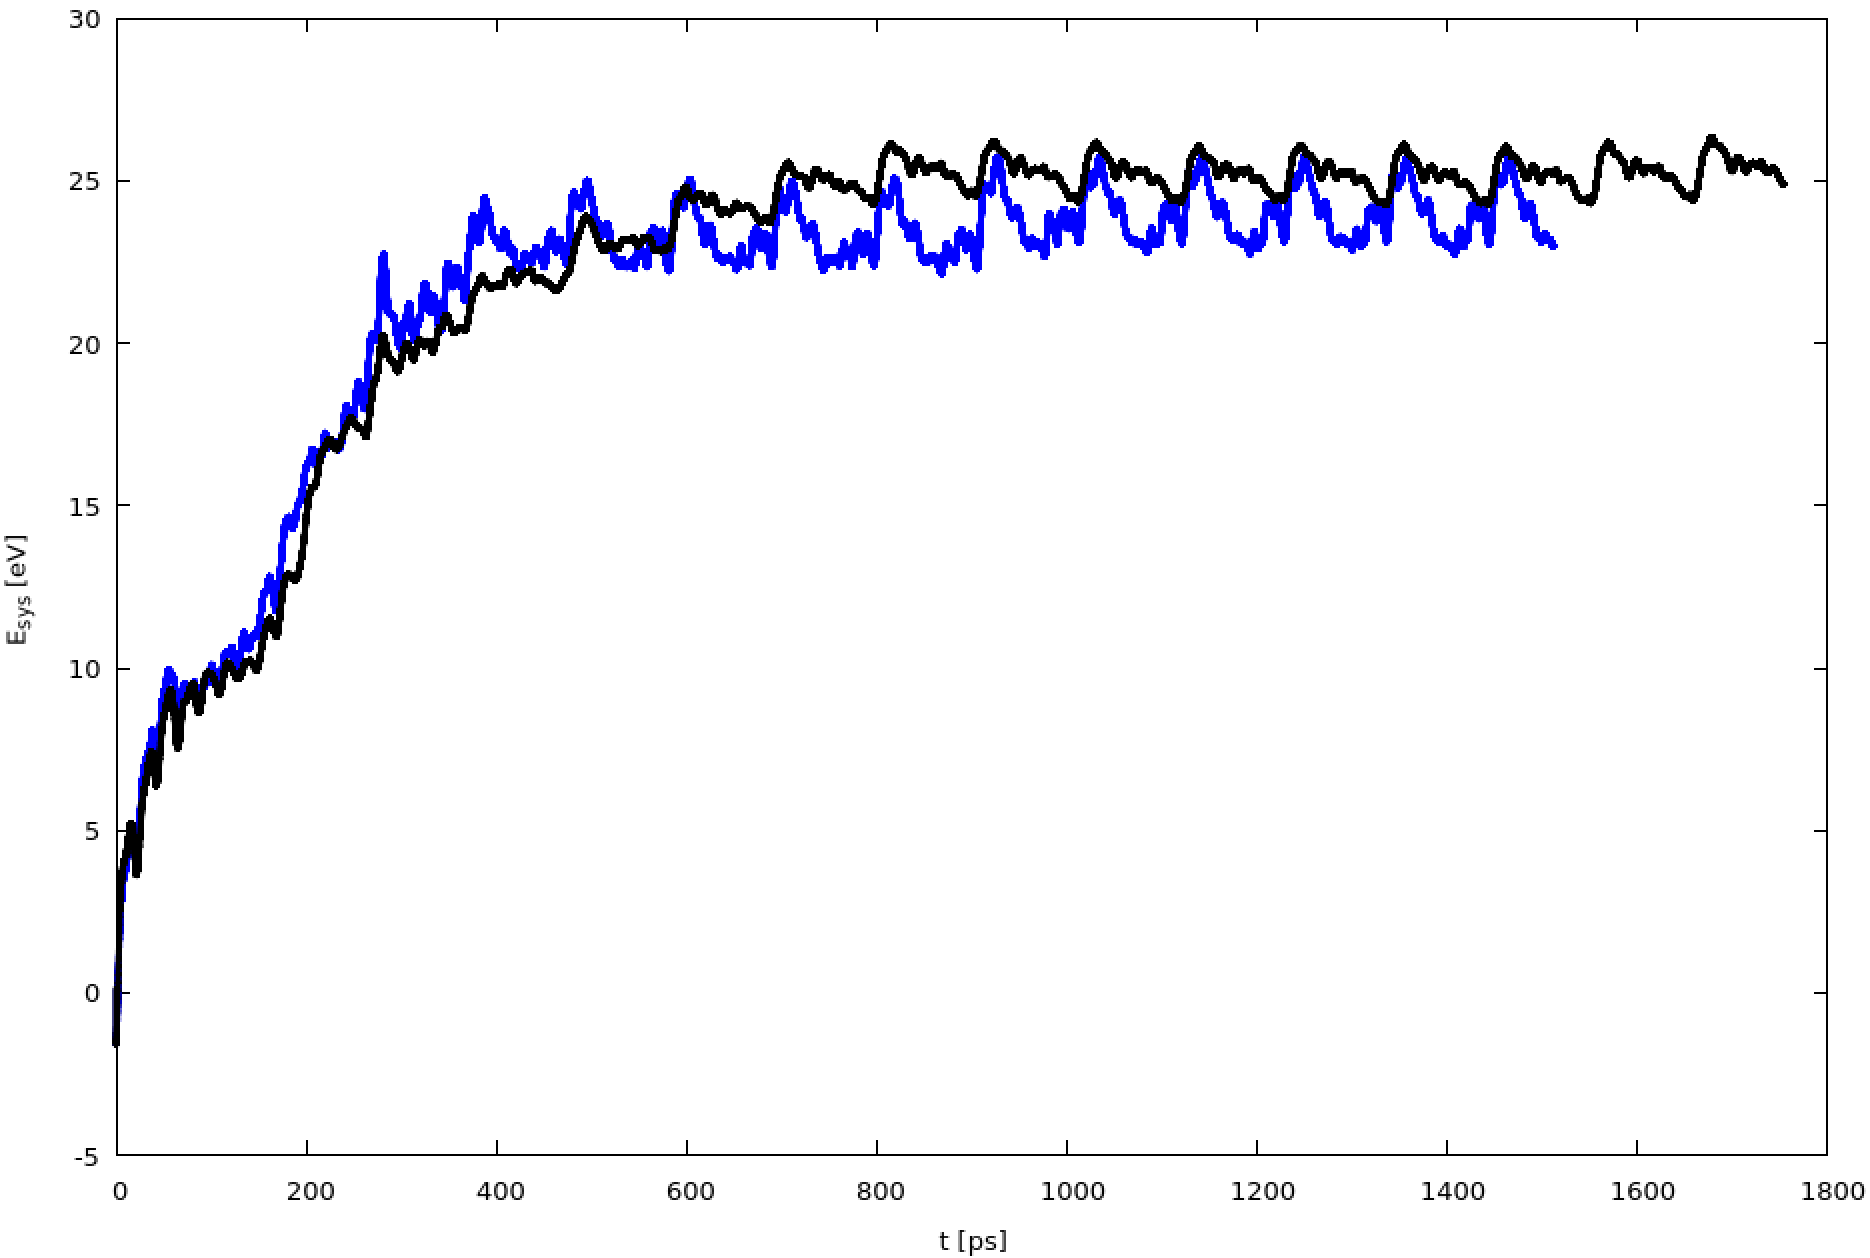
\includegraphics[width=0.6\textwidth]{figs/1_energy.png}
	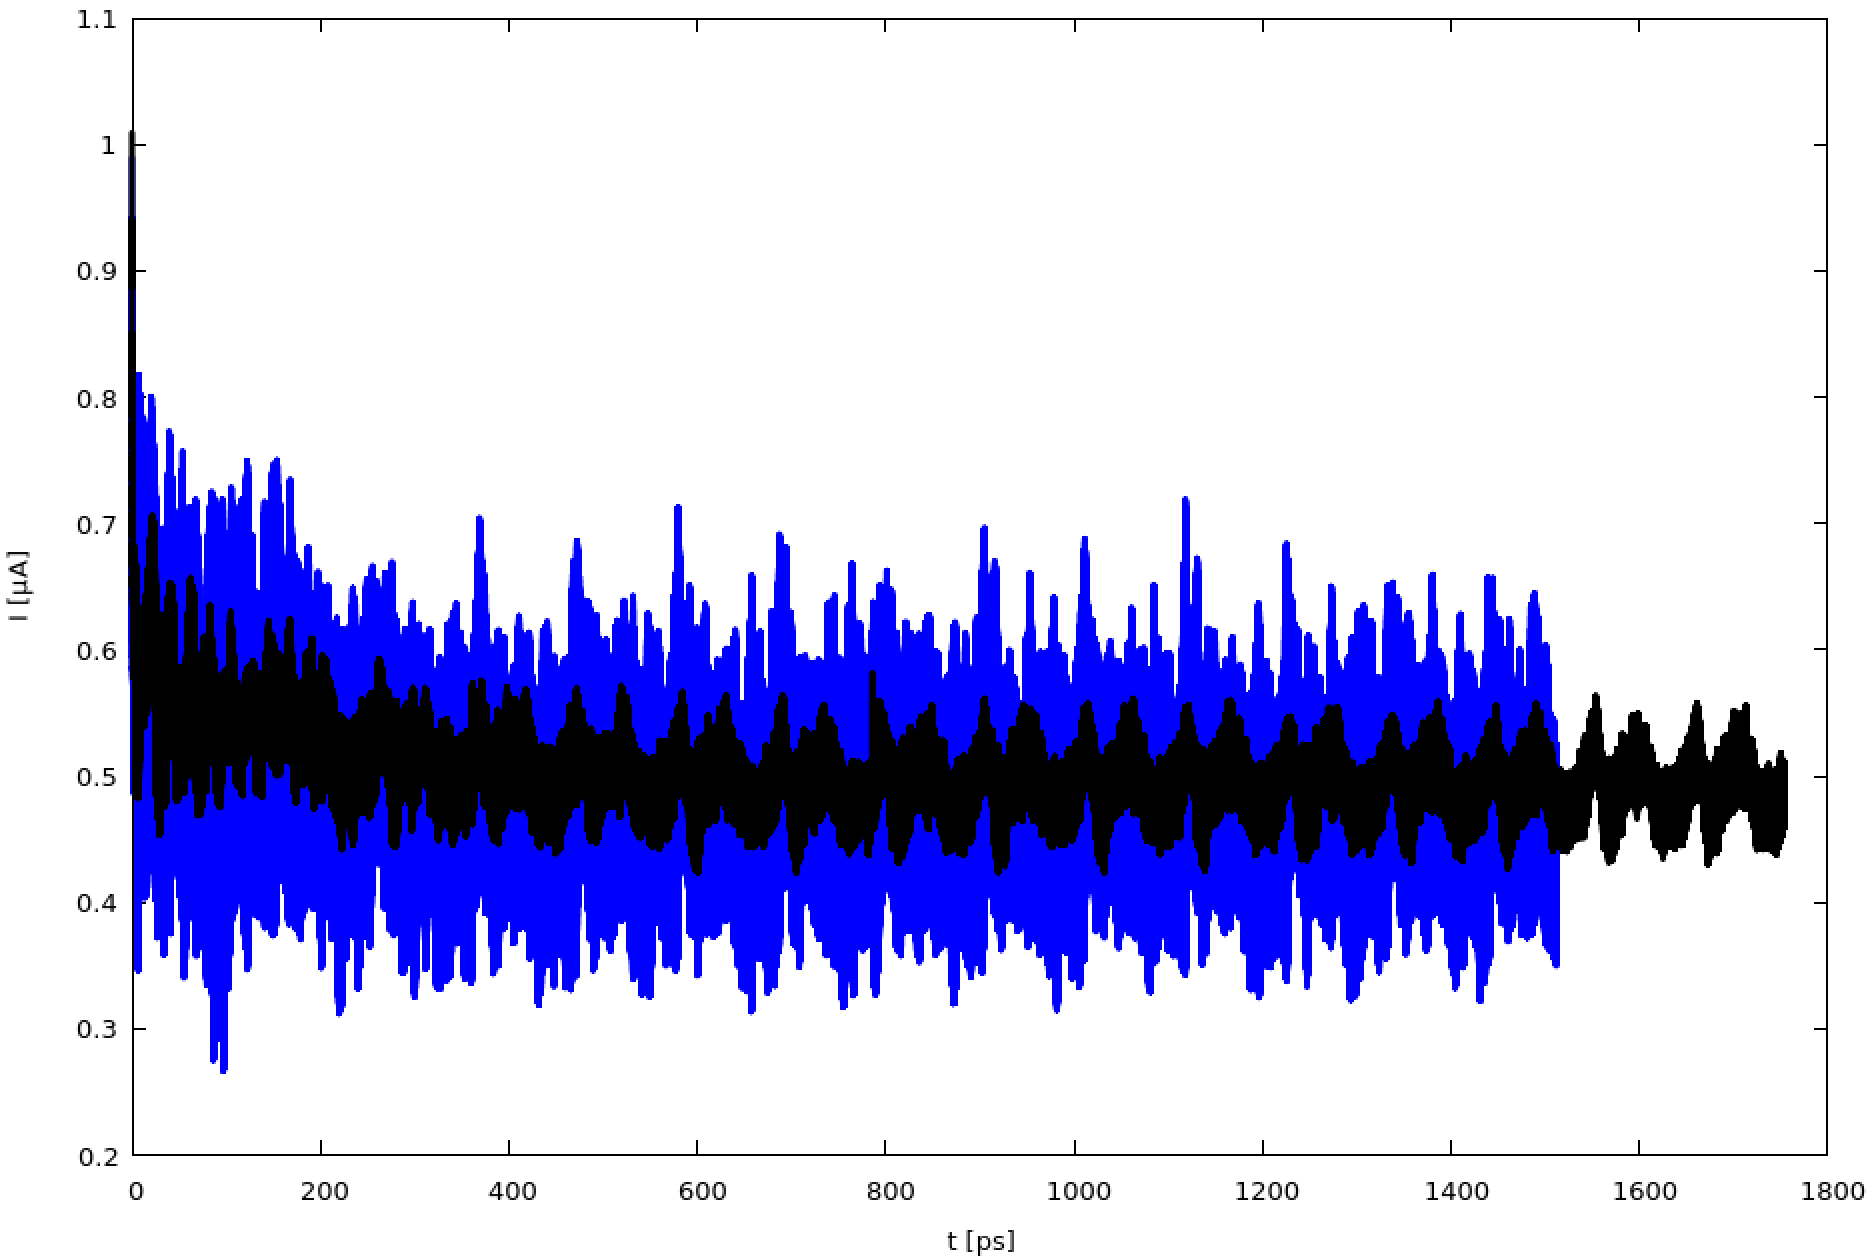
\includegraphics[width=0.6\textwidth]{figs/1_currents.png}
	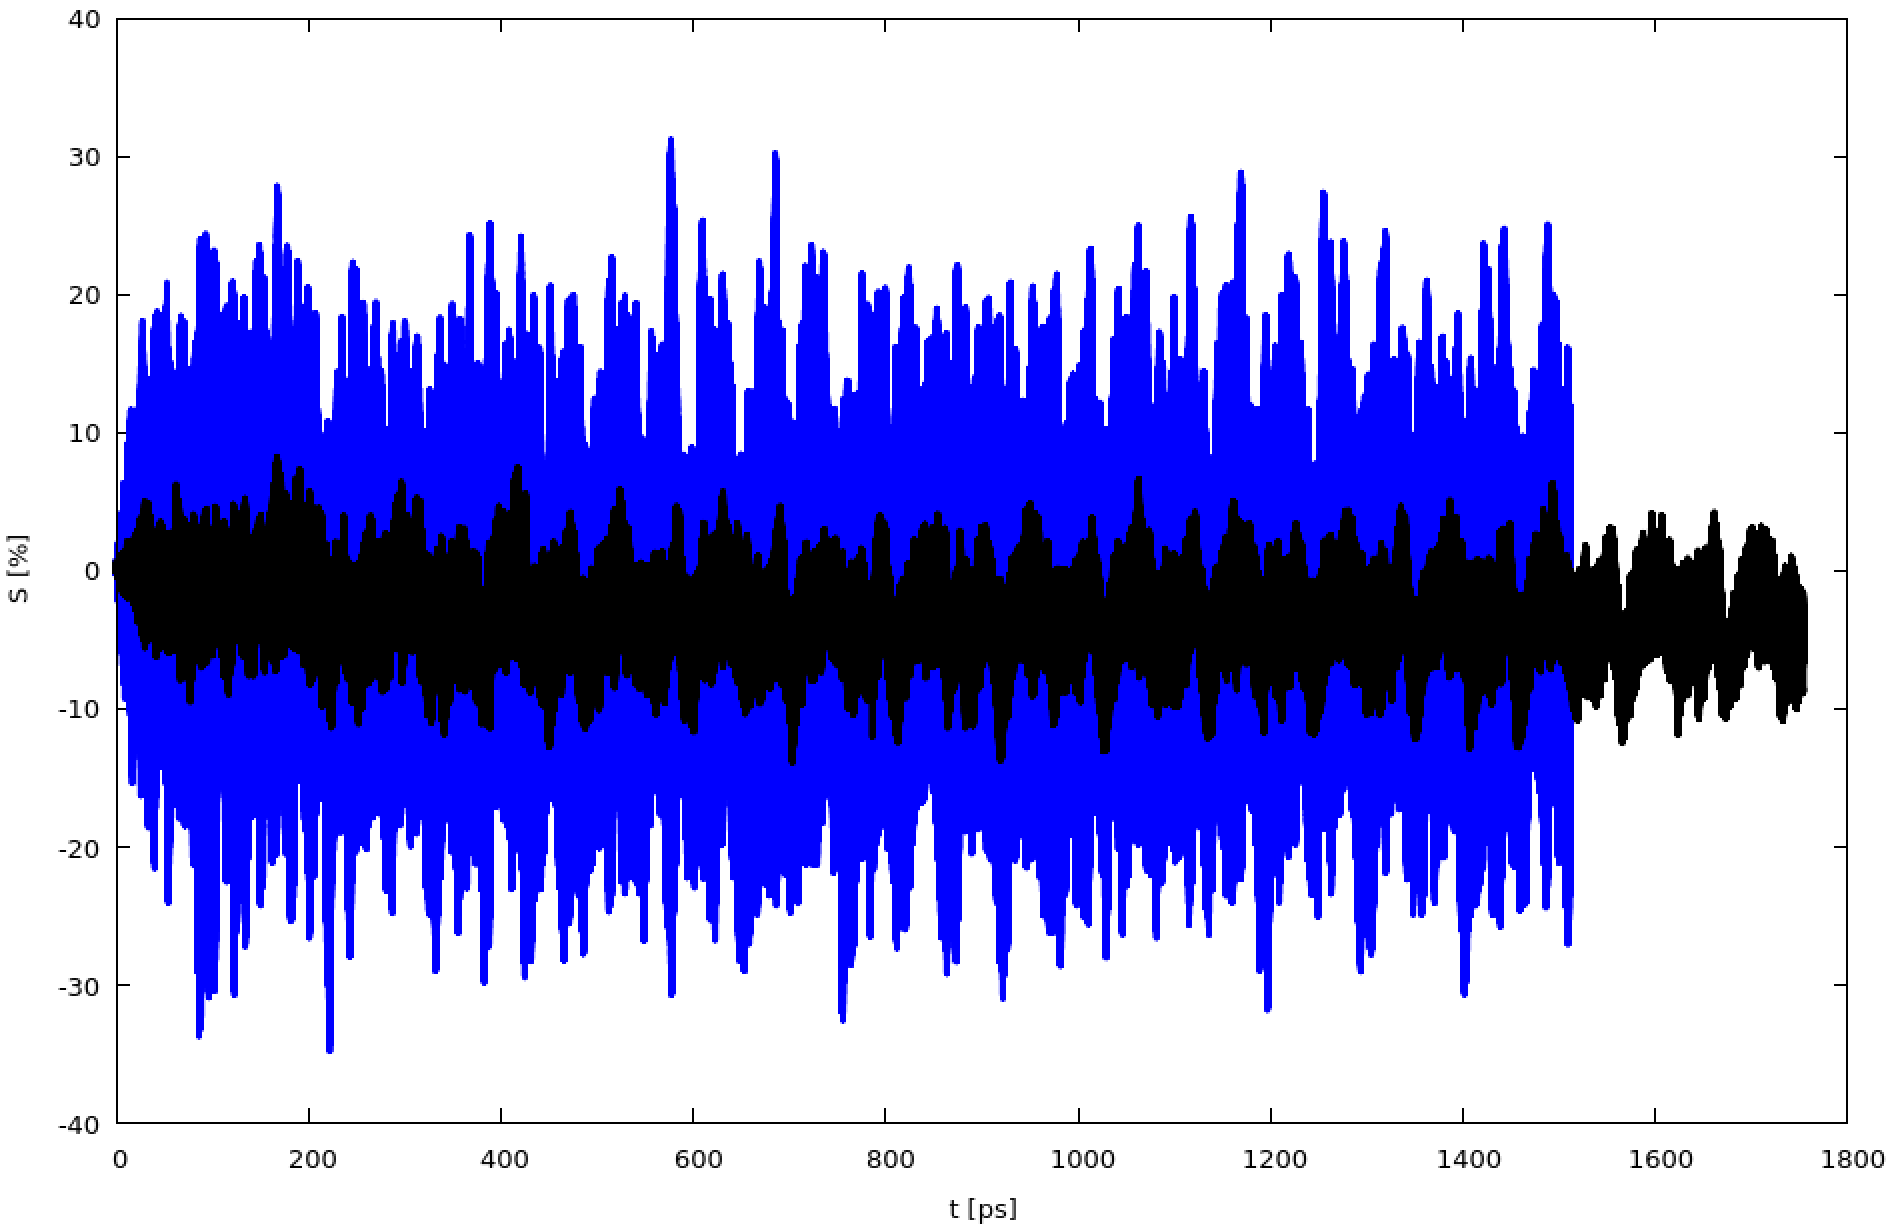
\includegraphics[width=0.6\textwidth]{figs/1_spin_selectivity.png}
	\caption{Time-dependent system energy, current, and spin selectivity. Ensemble-average over 31 trajectories (blue) and 401 trajectories (black).}\label{fig:1_E_I_S}
\end{figure}\\
The Fourier transform of the charge current (\cref{fig:1_FT}) shows peaks at well-defined frequencies, meaning the behavior of the current is periodic.
\begin{figure}[!h]
	\centering
	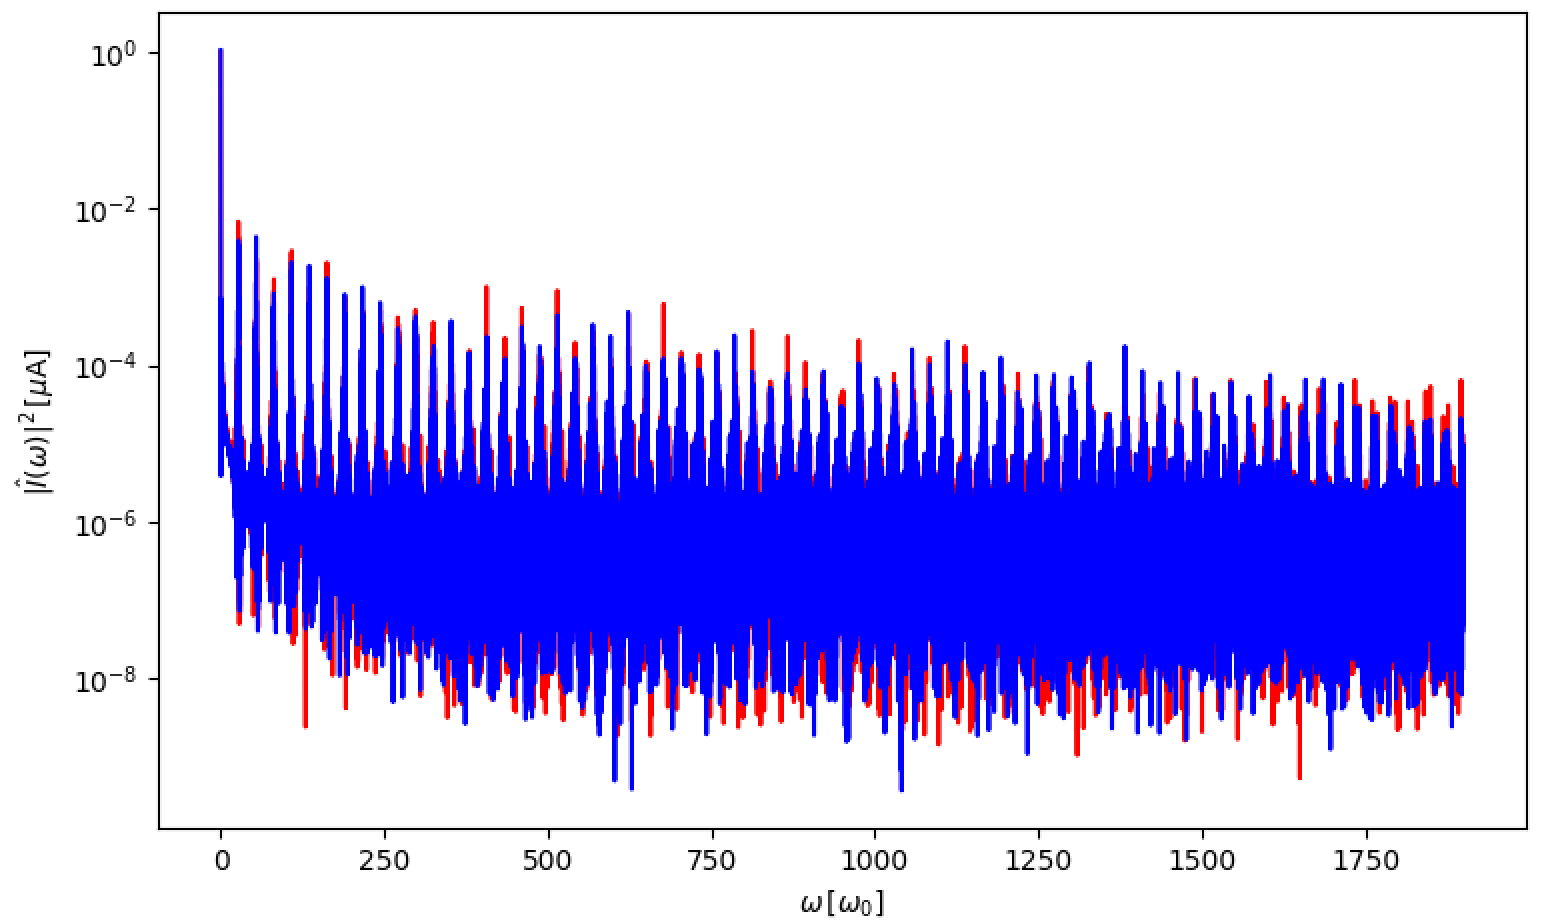
\includegraphics[width=0.45\textwidth]{figs/1_ft_ens_1.png}
	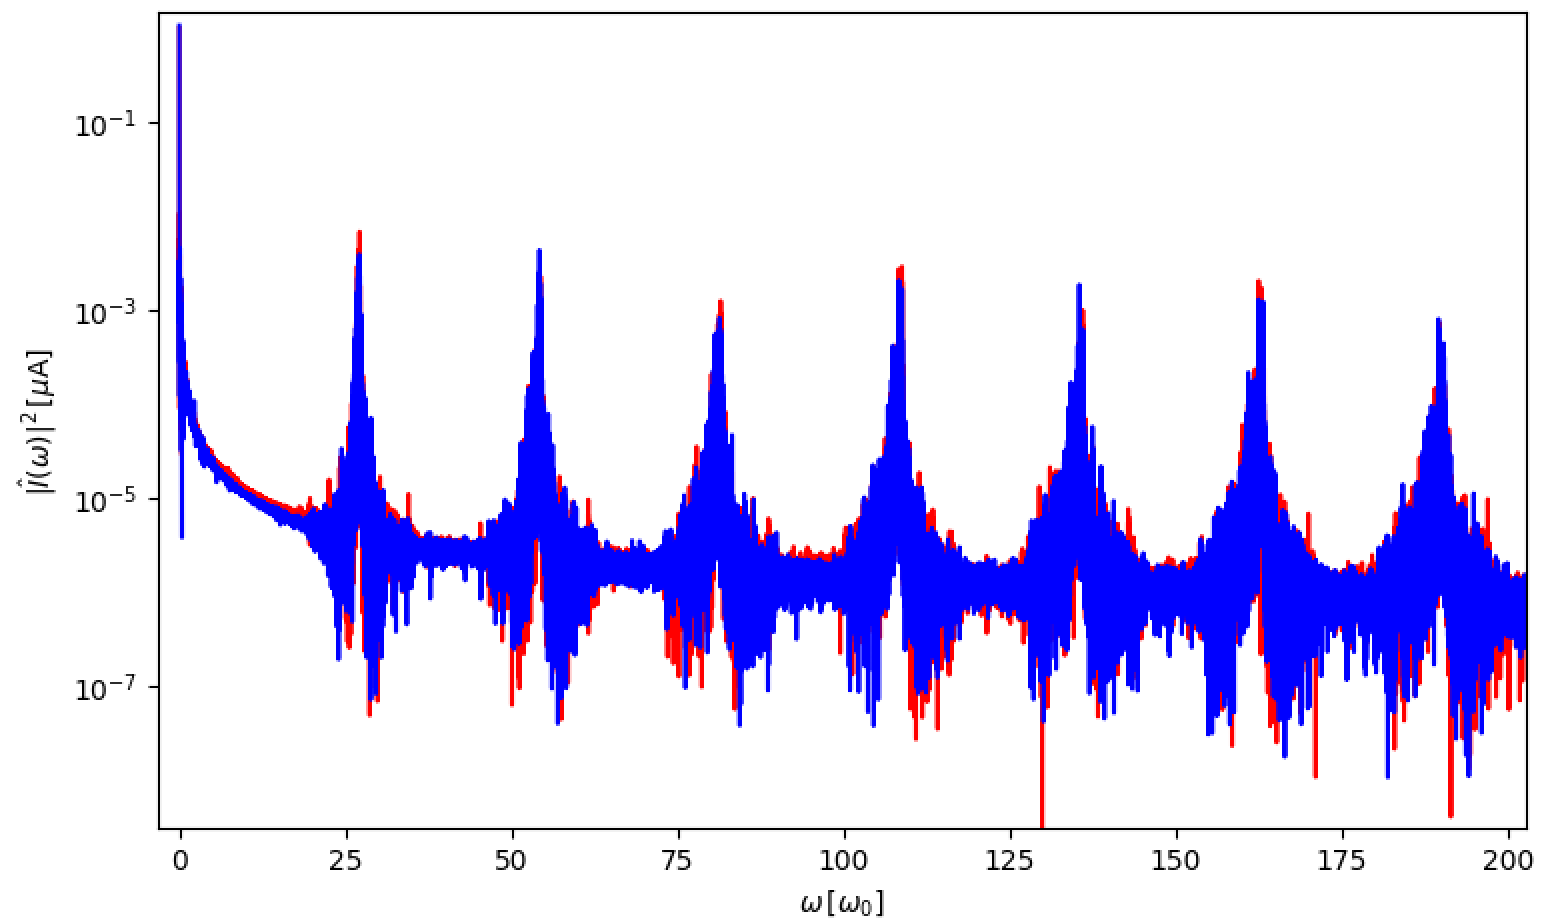
\includegraphics[width=0.45\textwidth]{figs/1_ft_ens_2.png}
	\caption{Fourier transform of the current: Full spectrum (top) and selected frequency range (bottom). All plots are obtained from the ensemble-averaged current for 401 trajectories.}\label{fig:1_FT}
\end{figure}\\
The ensemble-averaged charge currents $I_+,I_-$ are time-averaged over several oscillation periods in the system energy. The end points of the time interval over which the average is obtained are depicted by red lines in \cref{fig:1_E_tint}. 
\begin{figure}[!h]
	\centering
	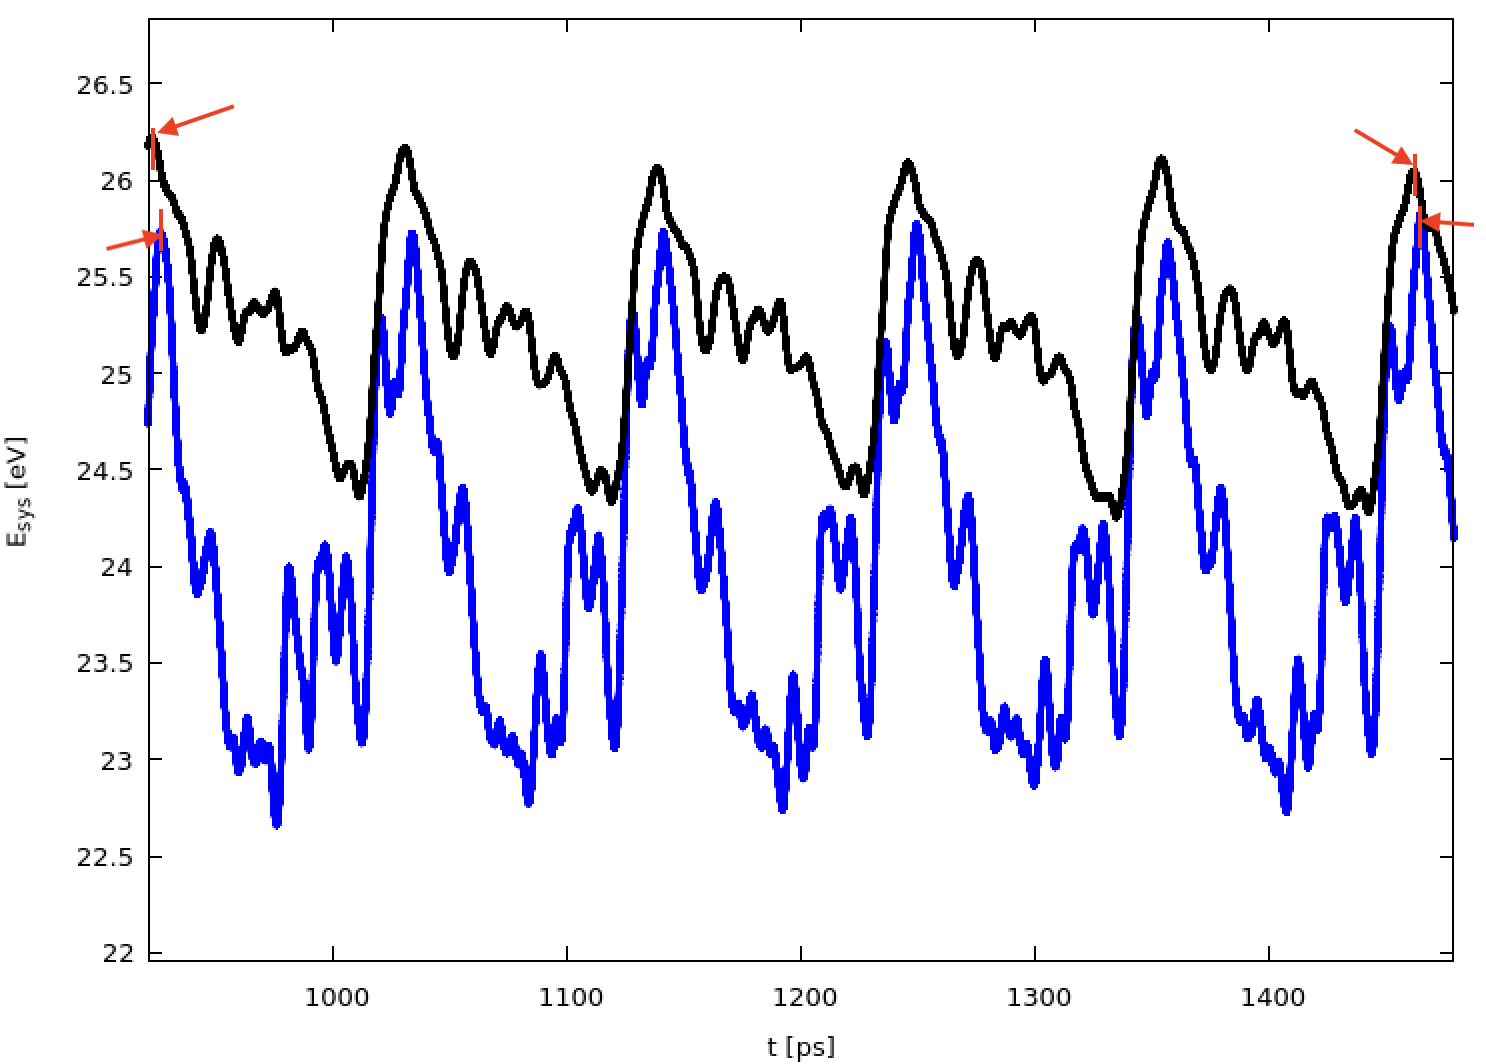
\includegraphics[width=0.6\textwidth]{figs/1_energy_zoom.png}
	\caption{Time interval for comparison of time-averages of ensemble-averaged currents for varying number of trajectories.}\label{fig:1_E_tint}
\end{figure}\\
The table below shows a comparison of the time-averages of currents for ensemble-averages over 31 and 401 trajectories. The standard errors on the ensemble-average (ens.) and on the time-average have been separated. 
\begin{table}[!h]
	\centering
	\begin{small}
		\begin{tabular}{cccc}
			\toprule
			Trajectories & $\langle \bar{I}_+ \rangle \, [\SI{}{\micro\ampere}]$ & $\langle \bar{I}_- \rangle \, [\SI{}{\micro\ampere}]$ & $S= \frac{\langle \bar{I}_+ \rangle-\langle \bar{I}_- \rangle}{\langle \bar{I}_+ \rangle+\langle \bar{I}_- \rangle}\, [\%]$\\
			\midrule
			31 & $0.9780\pm 0.0004\mathrm{(ens.)}\pm 0.0001\mathrm{(time)}$ & $1.0528\pm 0.0004\mathrm{(ens.)}\pm 0.0001\mathrm{(time)}$ & $-3.69 \pm 0.03\mathrm{(comb.)}$ \\
			401 & $1.01225\pm 0.0004 \mathrm{(ens.)}\pm 0.00003\mathrm{(time)}$ & $1.08545\pm 0.0004\mathrm{(ens.)}\pm 0.00003\mathrm{(time)}$ & $-3.49\pm 0.02\mathrm{(comb.)}$ \\
			\bottomrule
		\end{tabular}
	\end{small}
\end{table}
\clearpage
\subsection{Time-distribution of ensemble-averaged currents}
\Cref{fig:1_dist} shows the distribution of ensemble-averaged current within the time-interval $t\geq \SI{400}{\pico\second}$. This plot shows that the statistics of the time-dependence of the ensemble-averaged current resembles a normal distribution. This legitimates taking the time-average of the ensemble-averaged current. 
\begin{figure}[!h]
	\centering
	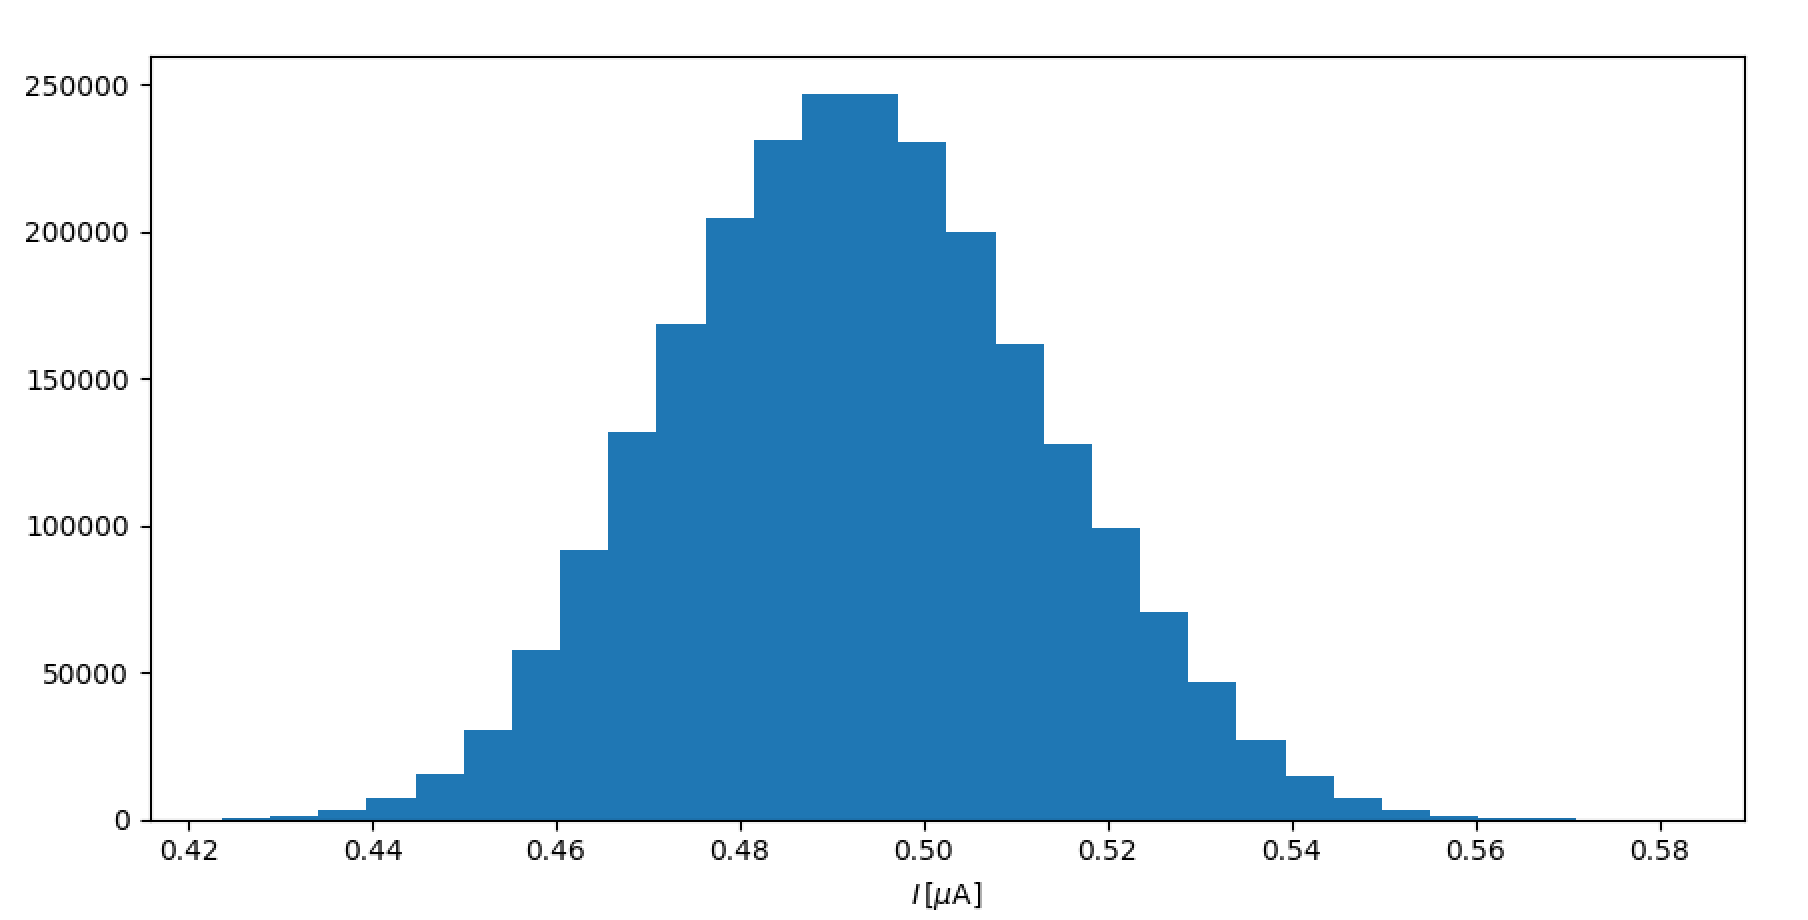
\includegraphics[width=0.7\textwidth]{figs/1_cur_t_stat.png}
	\caption{Distribution of ensemble-averaged current for time-interval considered in the time-average.}\label{fig:1_dist}
\end{figure}
Moving averages of the ensemble-averaged current and the therefrom obtained spin selectivity are shown in \cref{fig:1_mov_avg}. These reflect the quasi-periodicity of the current by being periodic in the long-time limit. The spin selectivity also picks up this time-periodicity. 
\begin{figure}[!h]
	\centering
	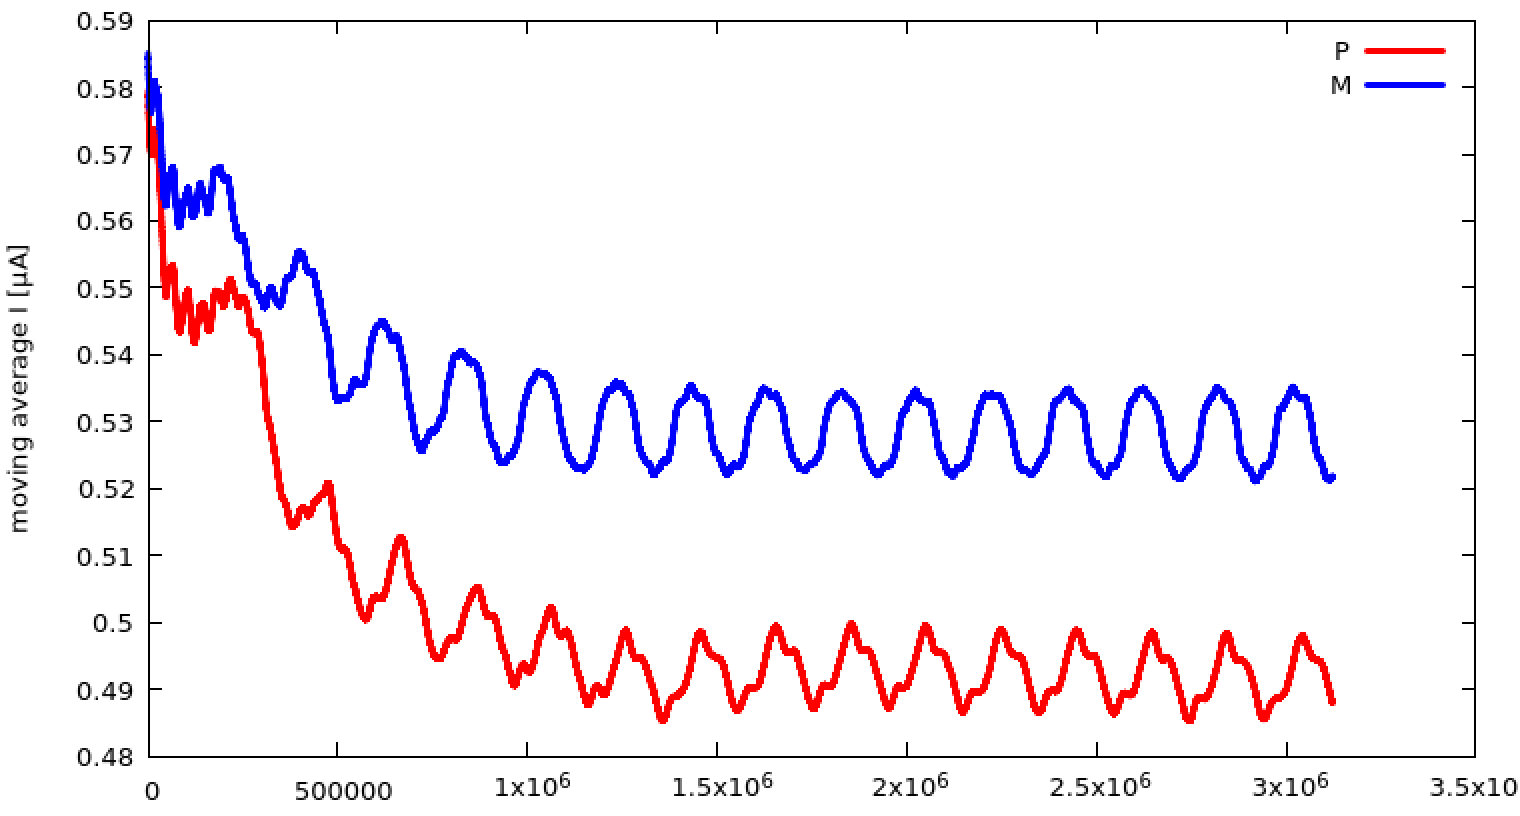
\includegraphics[width=0.6\textwidth]{figs/1_cur_mov_avg.png}
	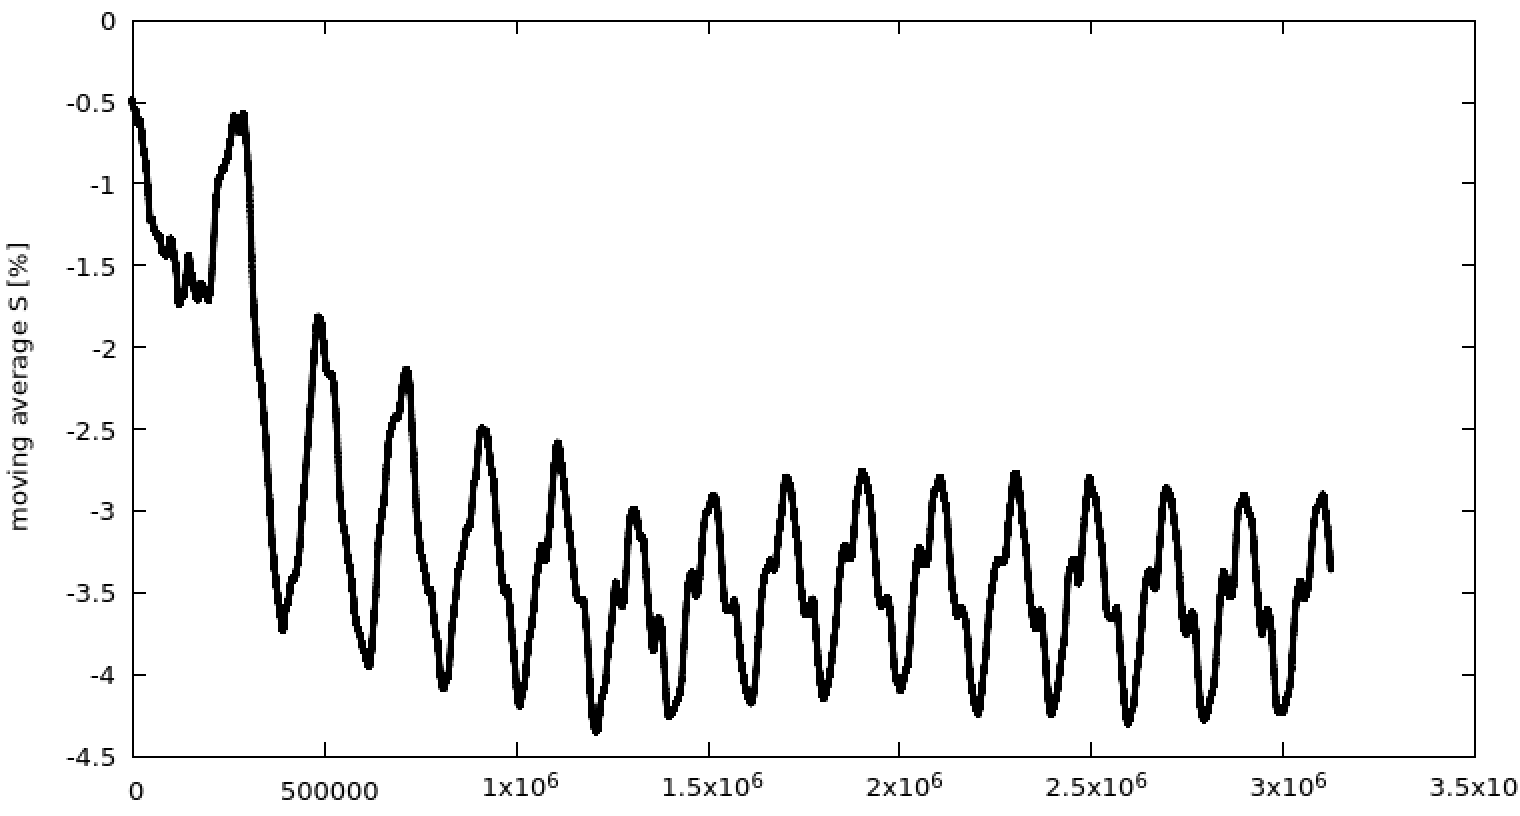
\includegraphics[width=0.6\textwidth]{figs/1_sp_mov_avg.png}
	\caption{Moving averages of ensemble-averaged current (top) and spin selectivity (bottom). Both for 401 trajectories.}\label{fig:1_mov_avg}
\end{figure}
\clearpage
\subsection{Ensemble-distribution of time-averaged currents}
\begin{figure}[!h]
	\centering
	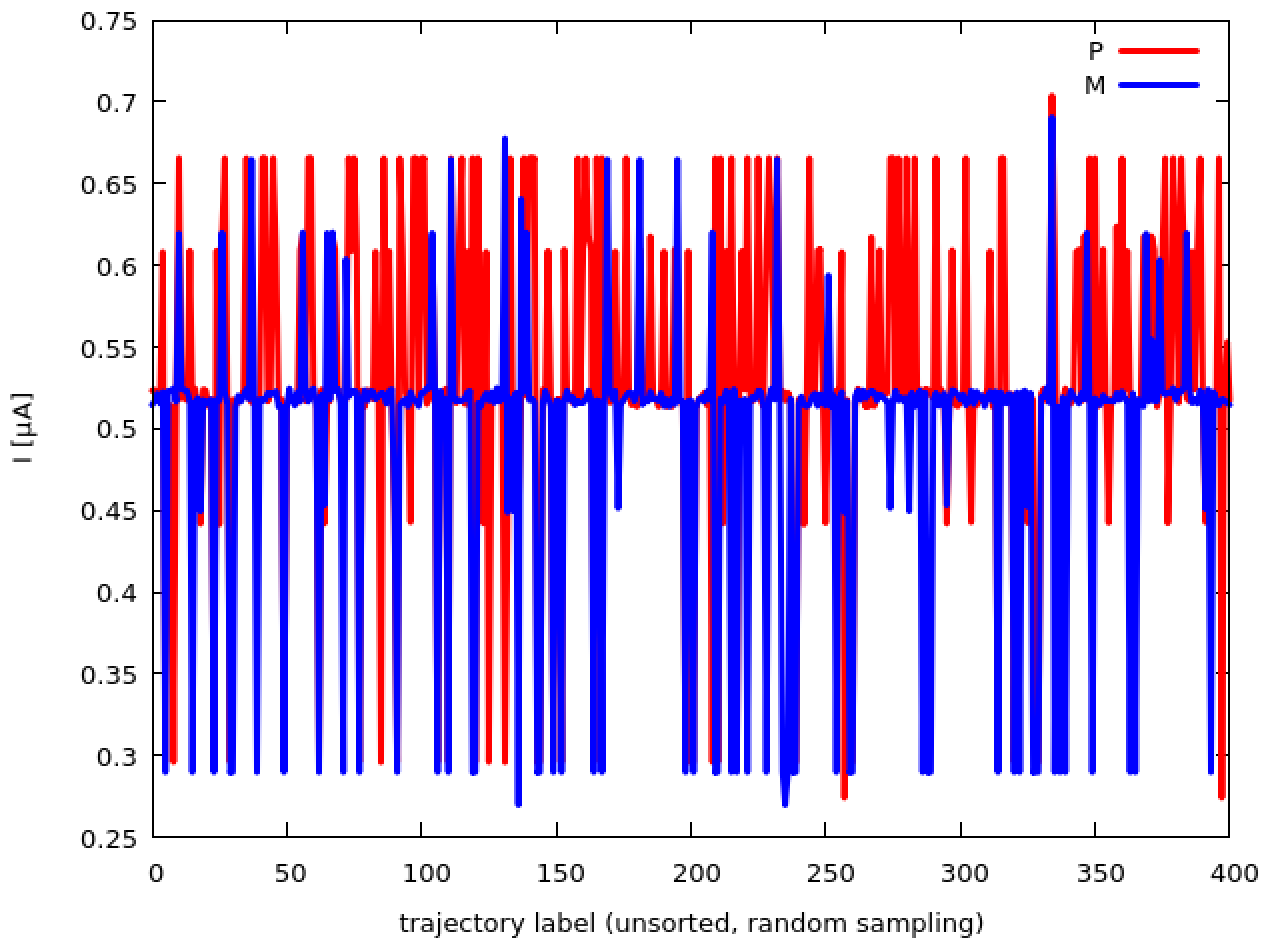
\includegraphics[width=0.6\textwidth]{figs/1_cur_traj.png}	
	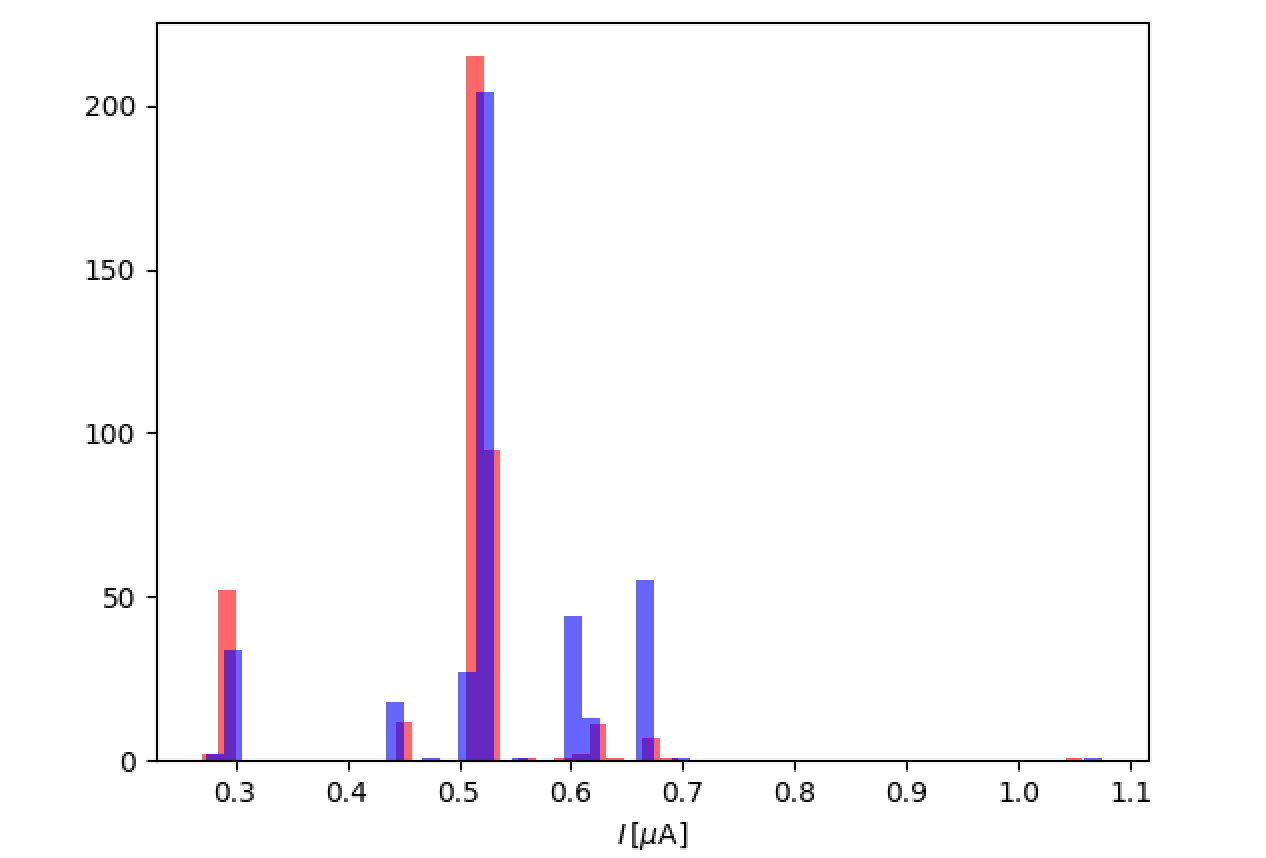
\includegraphics[width=0.6\textwidth]{figs/1_cur_stats.png}
	\caption{Average currents (time average taken over interval $[1.5,2]\,$ns) of the different trajectories (top).
	Histogram of time-averaged currents (bottom). The mean is at $\SI{0.495}{\micro\ampere}$.\\
	The problem is that there is a significant amount of outliers and thus that time-averaged currents do not follow a normal distribution for different initial conditions.}
\end{figure}
\begin{figure}[!h]
	\centering
	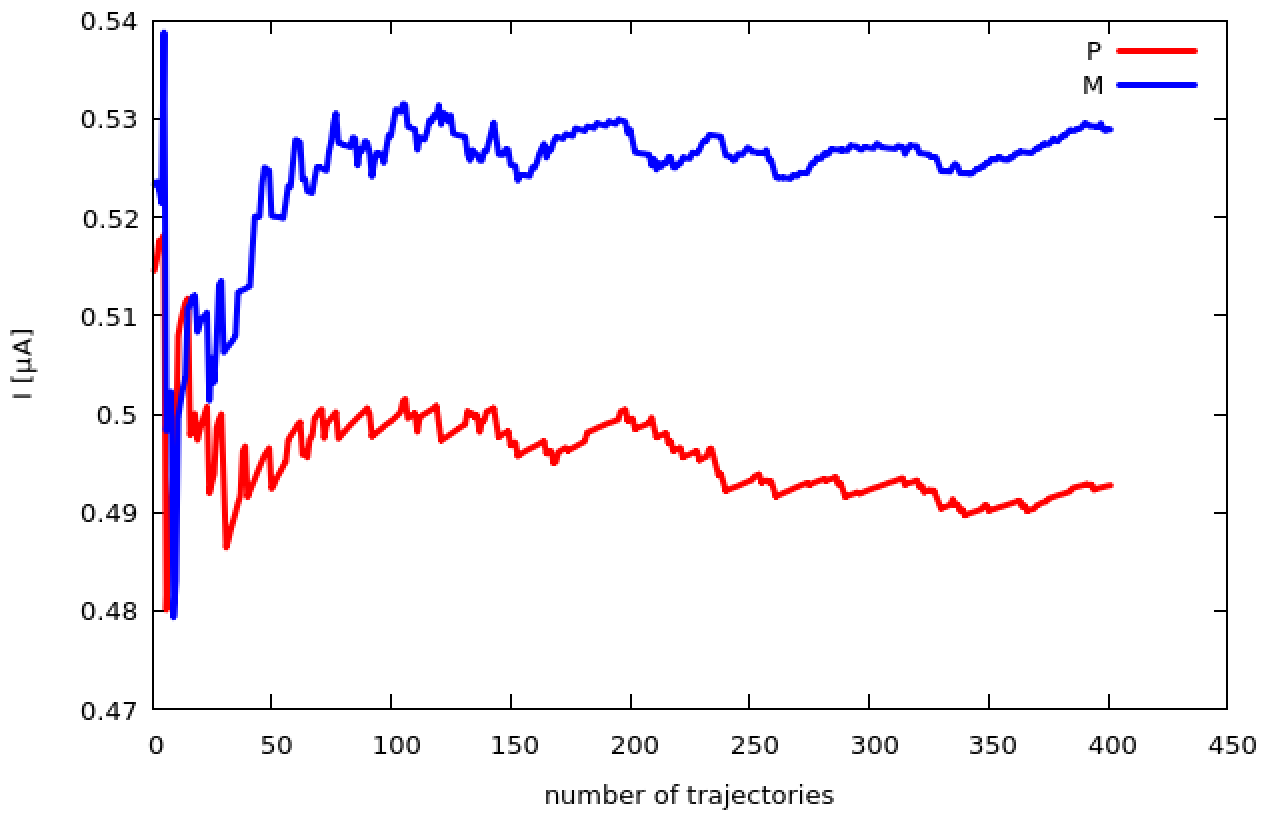
\includegraphics[width=0.6\textwidth]{figs/1_cur_nvar.png}
	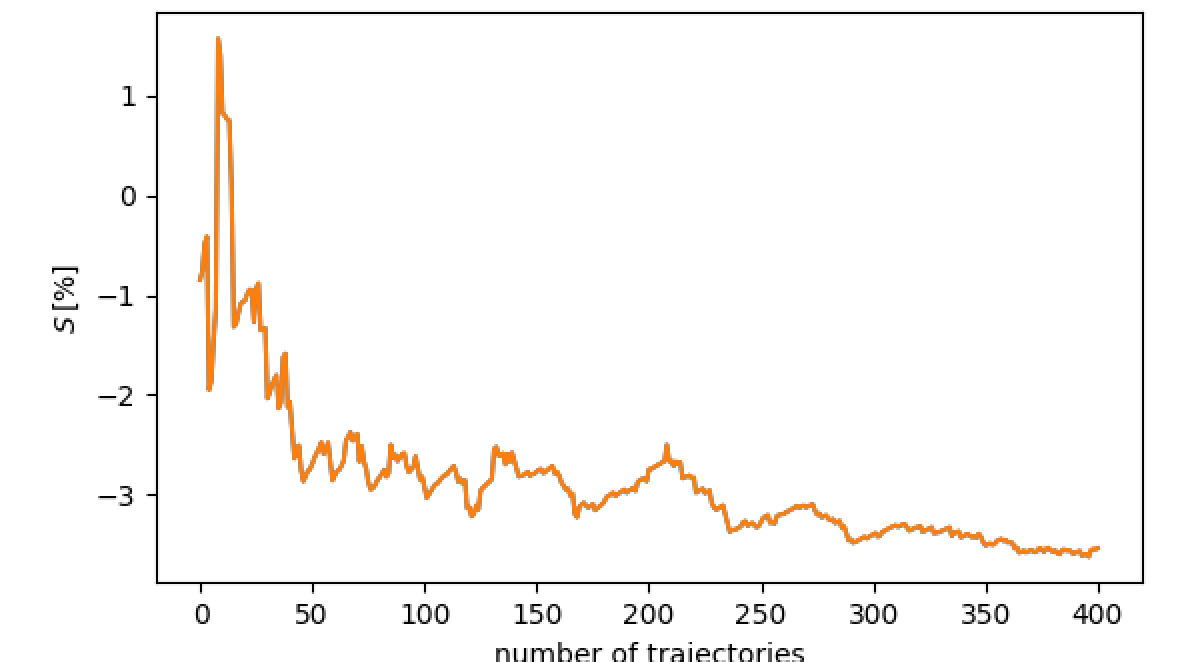
\includegraphics[width=0.6\textwidth]{figs/1_sp_nvar.png}
	\caption{ Ensemble-average of time-averaged currents varying number of trajectories (top) and spin selectivity (bottom).}
\end{figure}
\clearpage
\section{Analysis of trajectories: Stationary states and limit cycles}
\begin{figure}[!h]
	\centering
	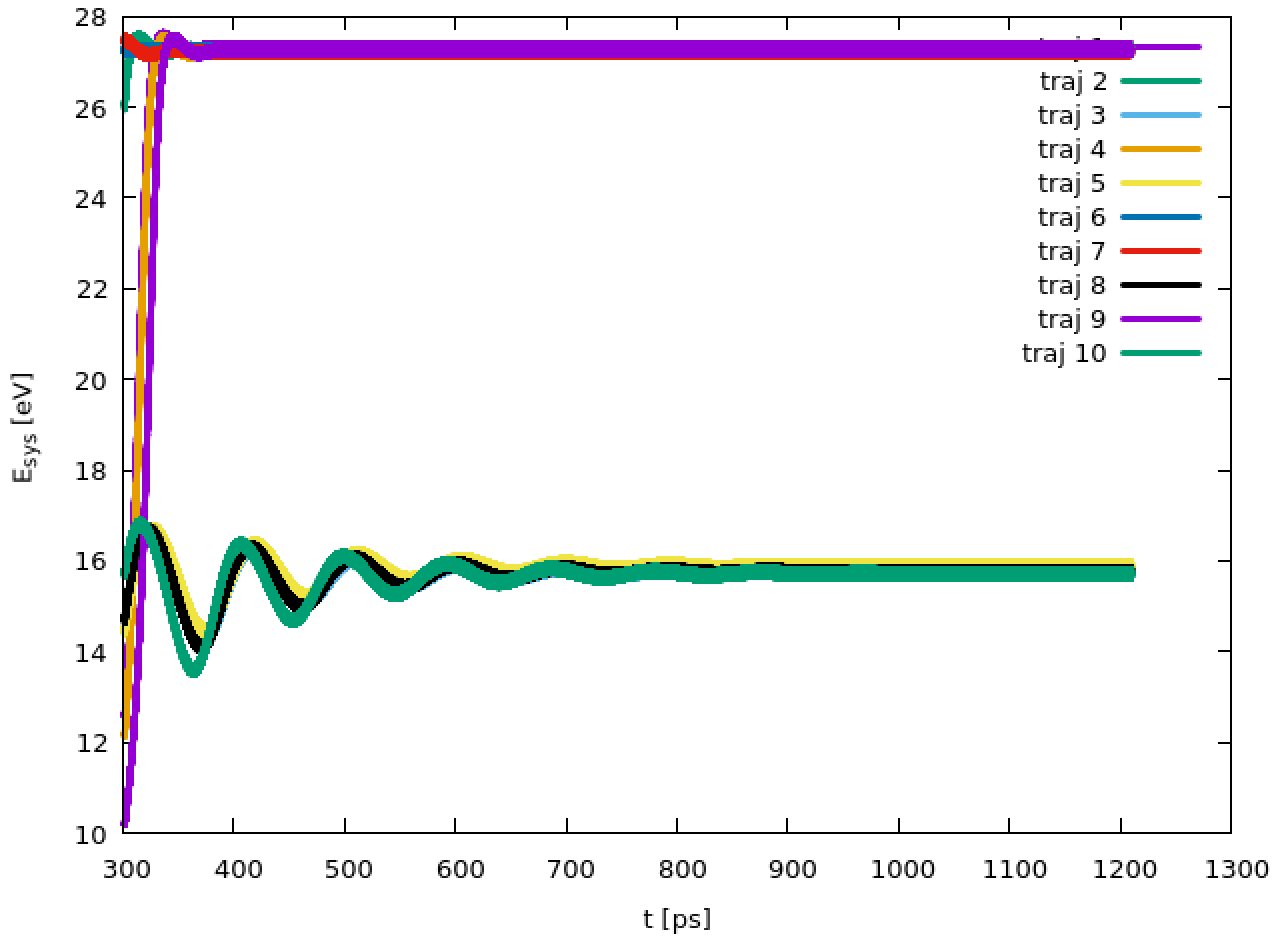
\includegraphics[width=0.7\textwidth]{figs/2_energy_trajs_1x4.png}
	\caption{$L=1\times 4$.}
\end{figure}
\begin{figure}[!h]
	\centering
	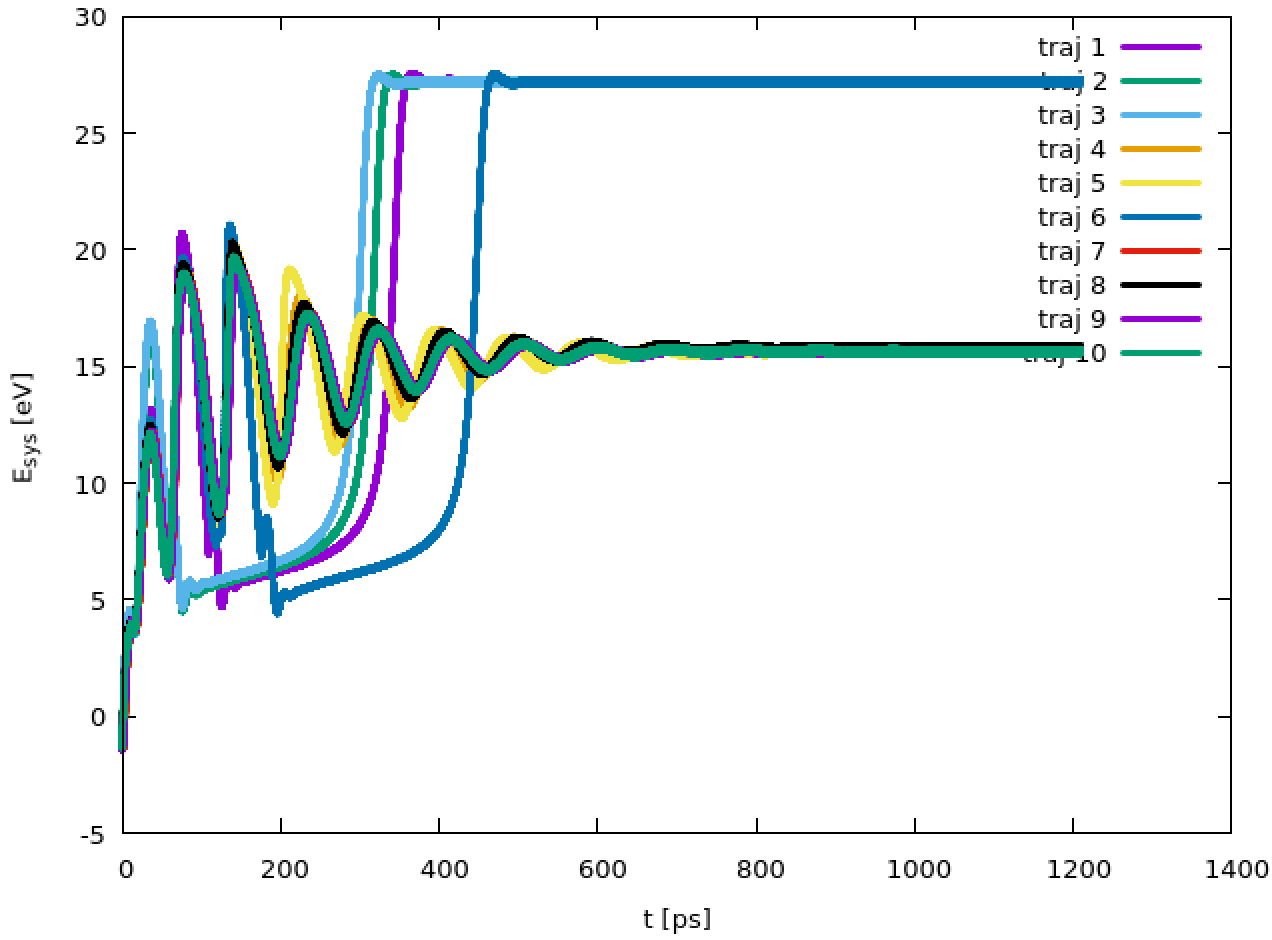
\includegraphics[width=0.7\textwidth]{figs/2_energy_trajs_2x2.png}
	\caption{$L=2\times 2$.}
\end{figure}
\begin{figure}[!h]
	\centering
	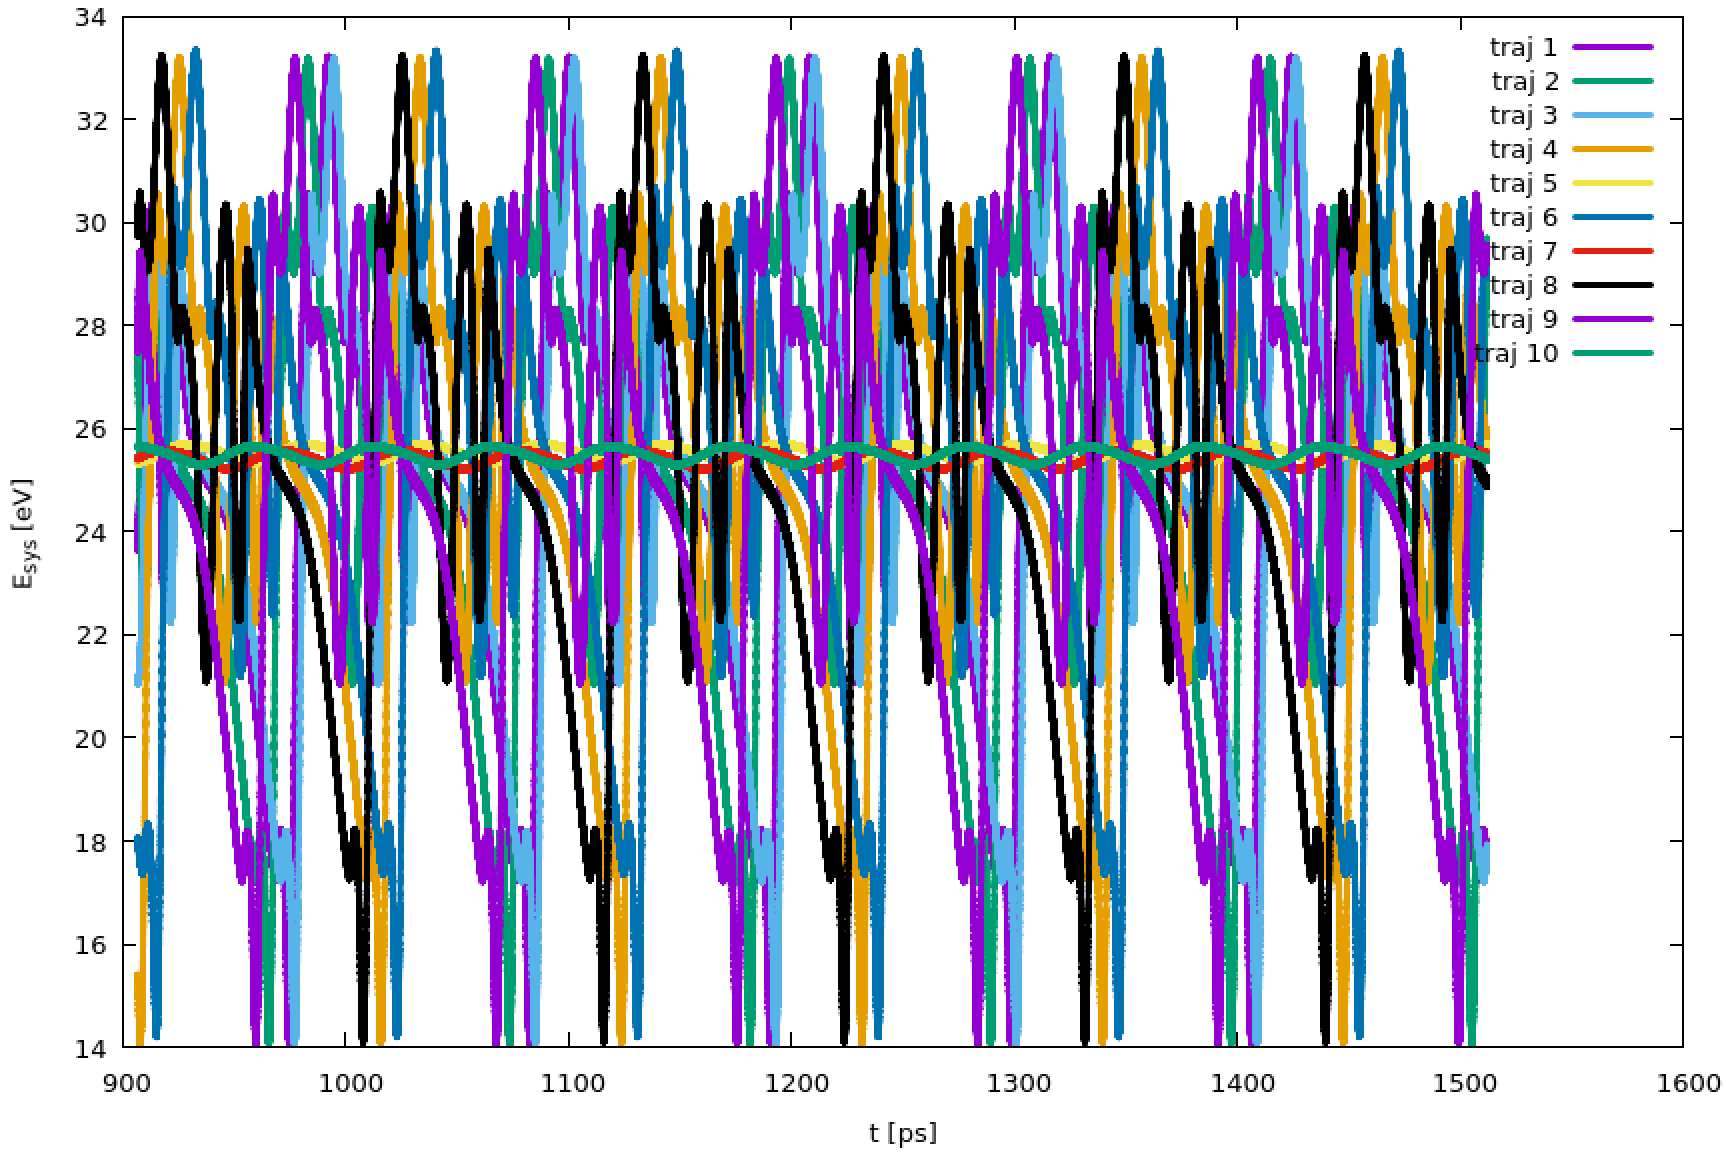
\includegraphics[width=0.7\textwidth]{figs/2_energy_trajs_1x5.png}
	\caption{$L=1\times 5$.}
\end{figure}
\begin{figure}[!h]
	\centering
	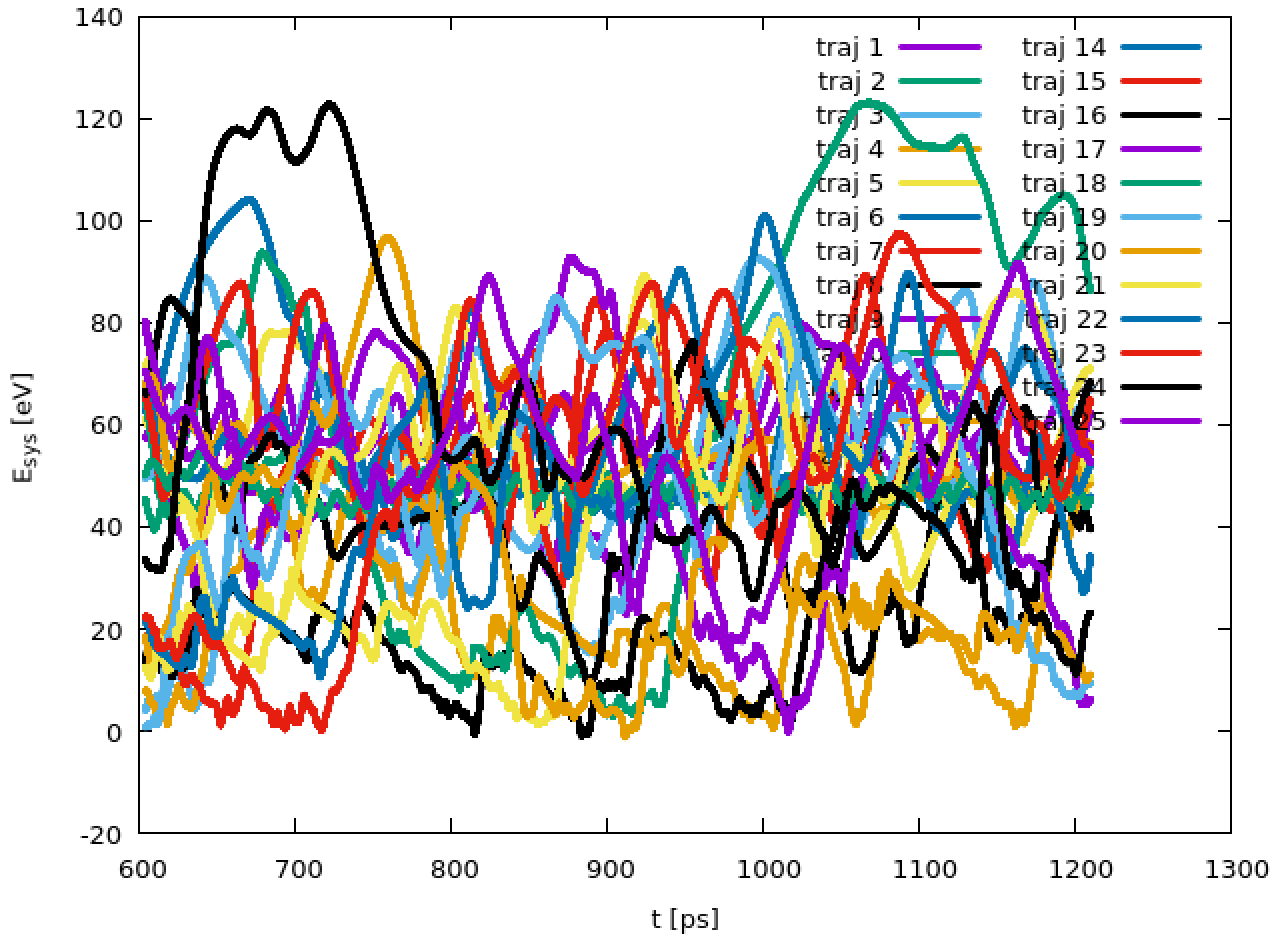
\includegraphics[width=0.7\textwidth]{figs/2_energy_trajs_1x6.png}
	\caption{$L=1\times 6$.}
\end{figure}
\clearpage
\section{How to obtain spin selectivity?}
Currents for $P=0.5$ and $P=-0.5$, spin selectivity, and system energy for selected trajectories ($L=1\times 5$). The idea was to compare the spin selectivity obtained from the time-average of the ensemble-averaged currents (in sec. 1) with an alternative approach: For each trajectory, compute the spin selectivity, and obtain time-average over an oscillation period, and then compare the trajectories with each other. The problem is that the current dynamics depends on the initial condition. Concretely, I would have to determine the initial and final times (for the time-average) for each trajectory individually. There is no simple way to automatize this task, because the trajectories look so differently. Examples are shown below. Each of the figures shows the current, spin selectivity and the system energy for different initial conditions. Another problem is that currents can cross the zero, and therefore the spin selectivity might be not well-defined.
\clearpage

\begin{figure}[!h]
	\centering
	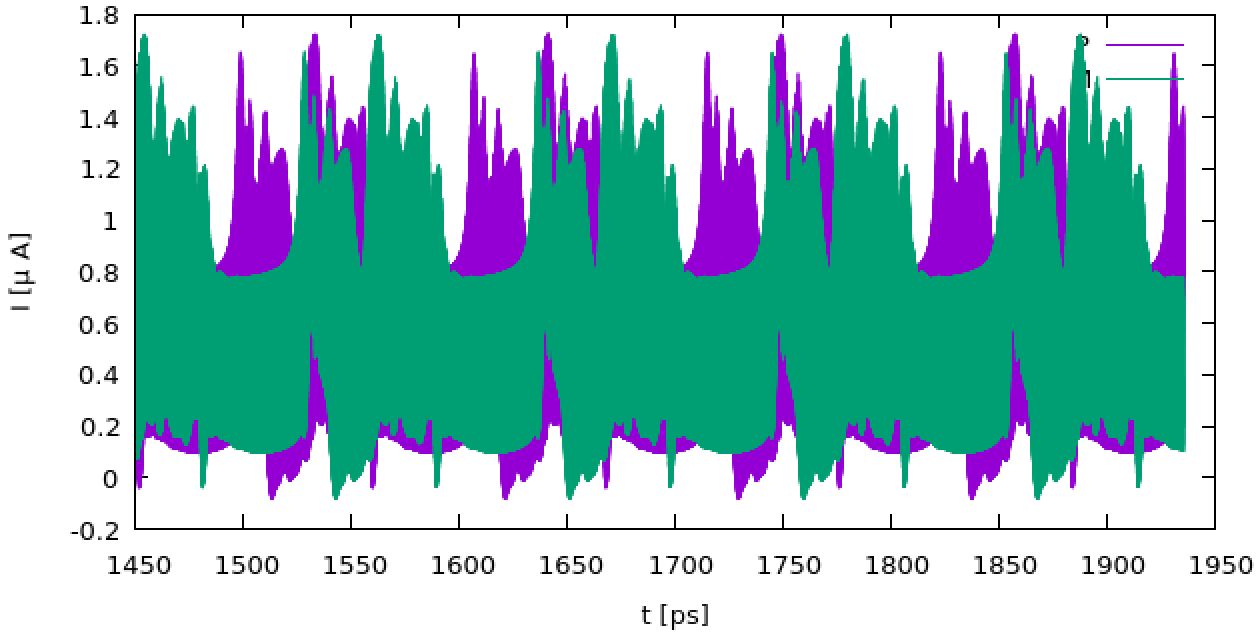
\includegraphics[angle=90,origin=c,width=0.35\textwidth]{figs/3_cur_1.png}
	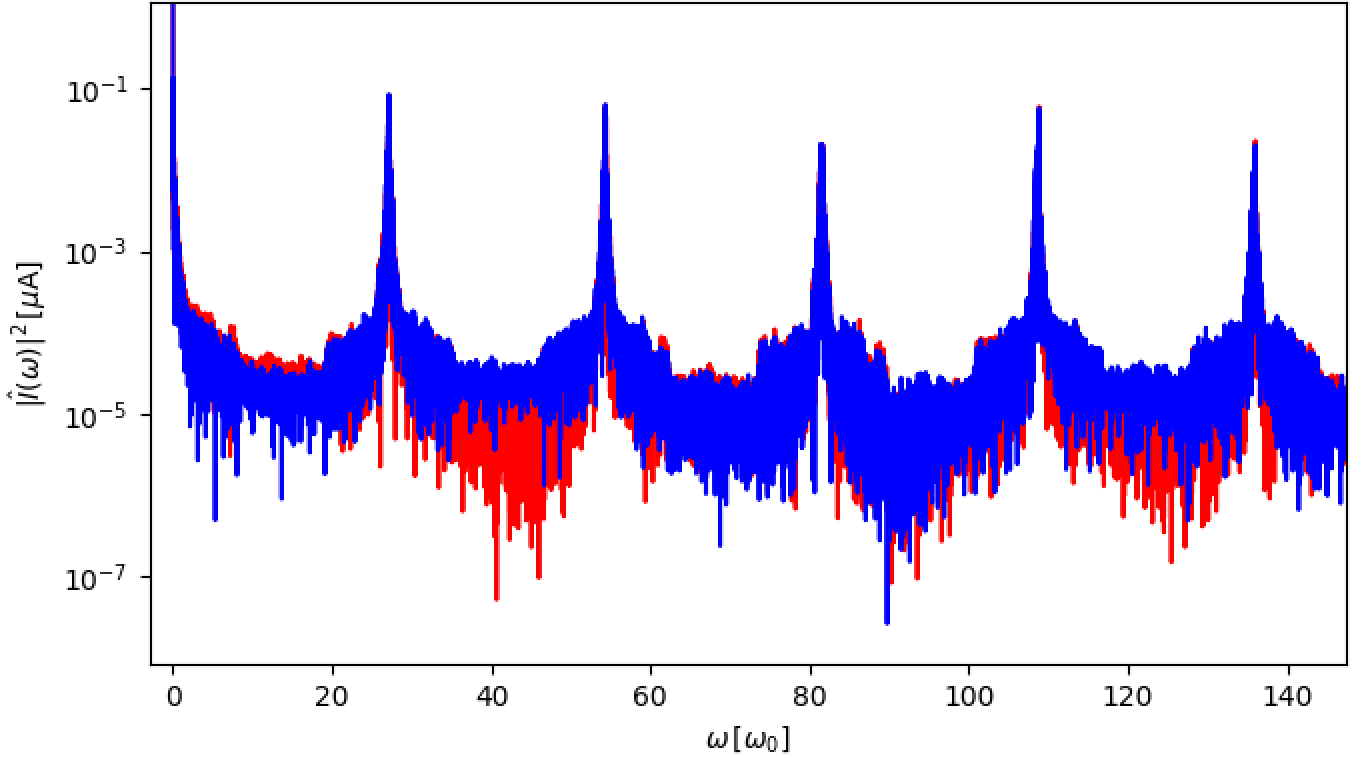
\includegraphics[angle=90,origin=c,width=0.35\textwidth]{figs/3_ft_1.png}
	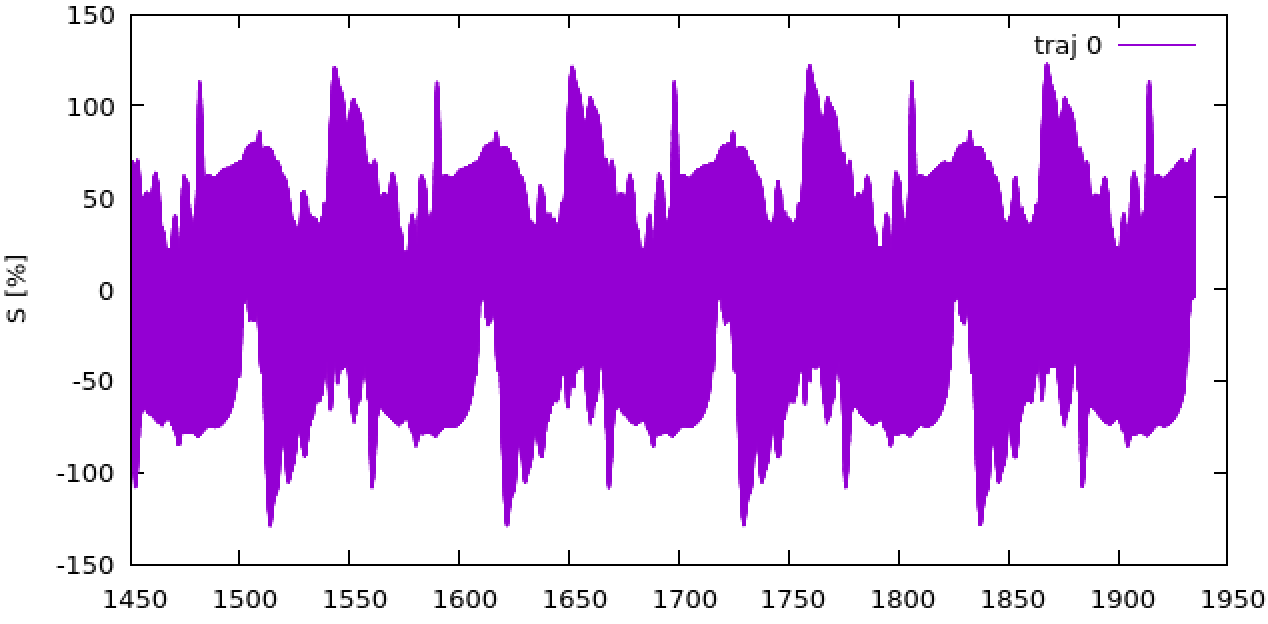
\includegraphics[angle=90,origin=c,width=0.35\textwidth]{figs/3_spin_selectivity_1.png}
	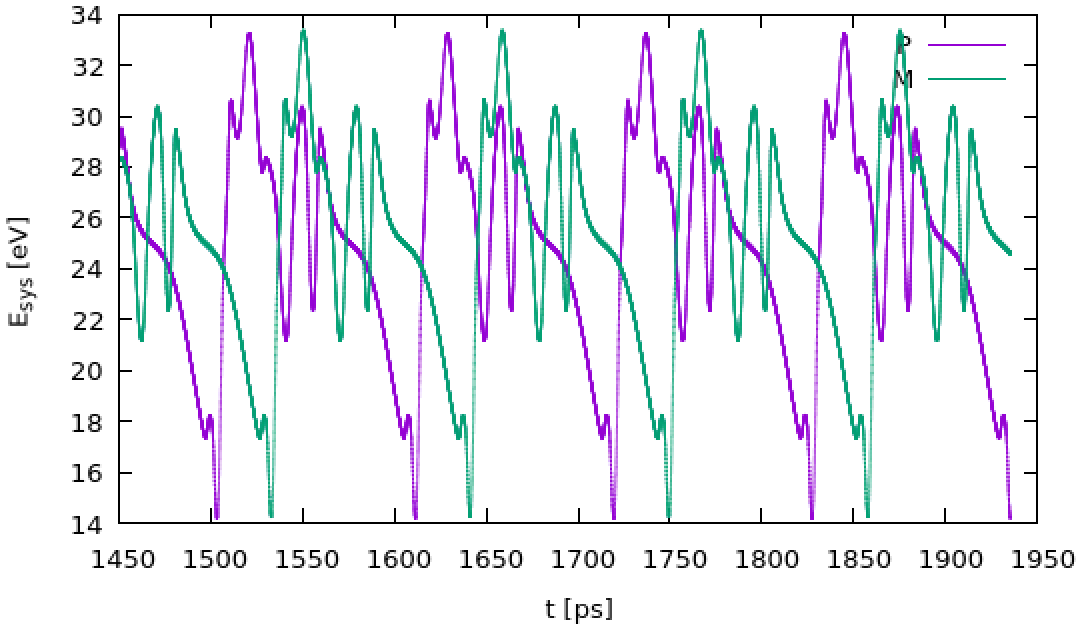
\includegraphics[angle=90,origin=c,width=0.35\textwidth]{figs/3_esys_1.png}
\end{figure}
\begin{figure}[!h]
	\centering
	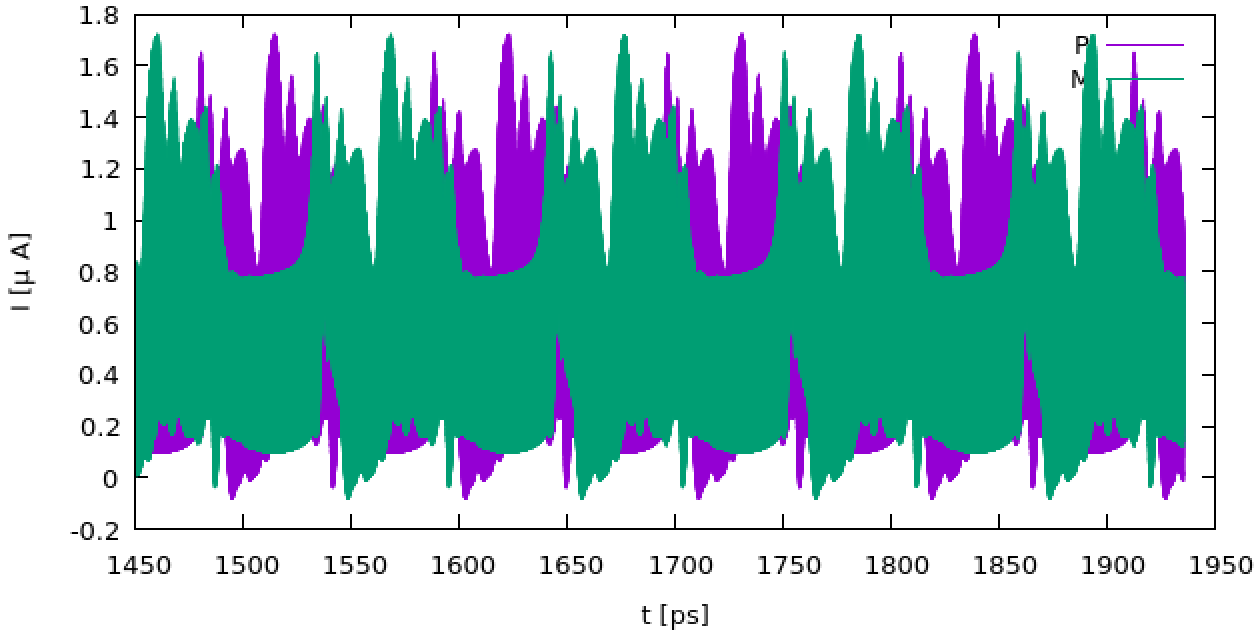
\includegraphics[angle=90,origin=c,width=0.35\textwidth]{figs/3_cur_2.png}	
	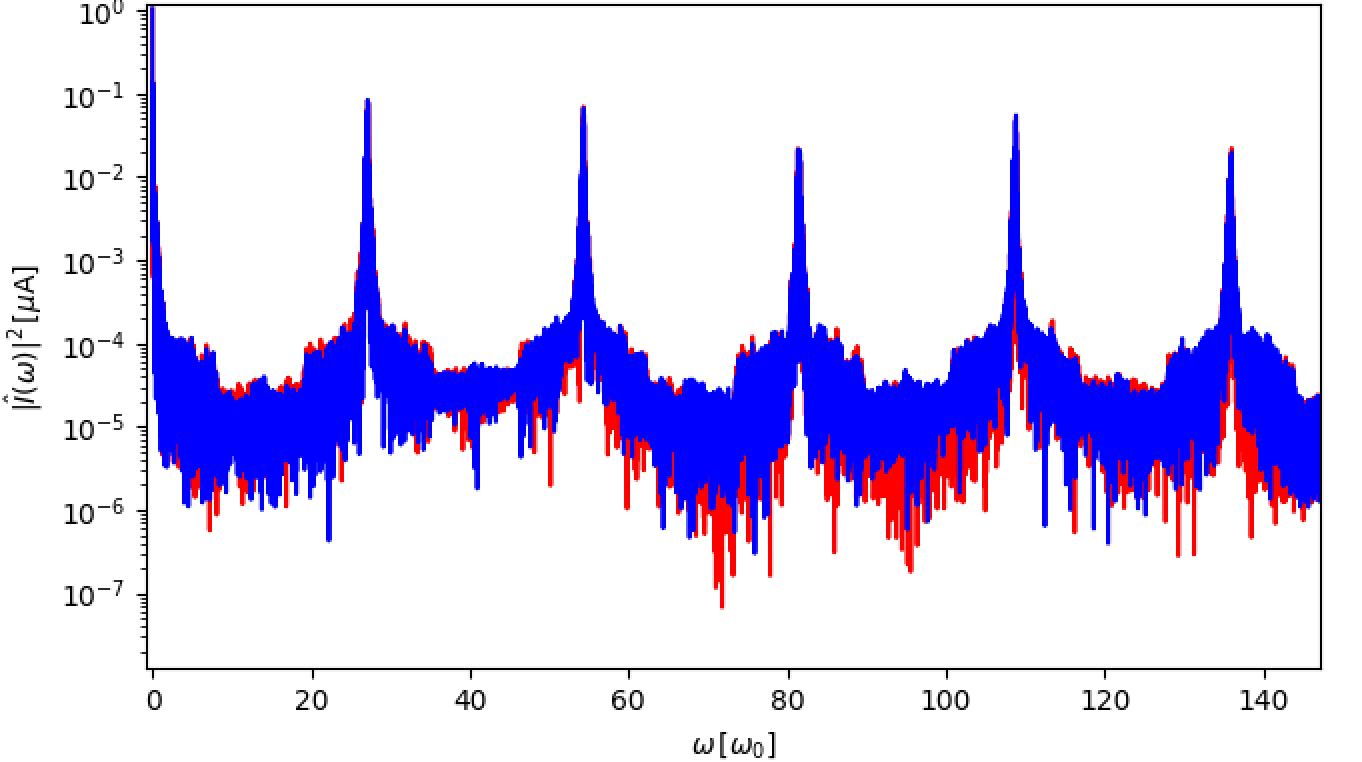
\includegraphics[angle=90,origin=c,width=0.35\textwidth]{figs/3_ft_2.png}
	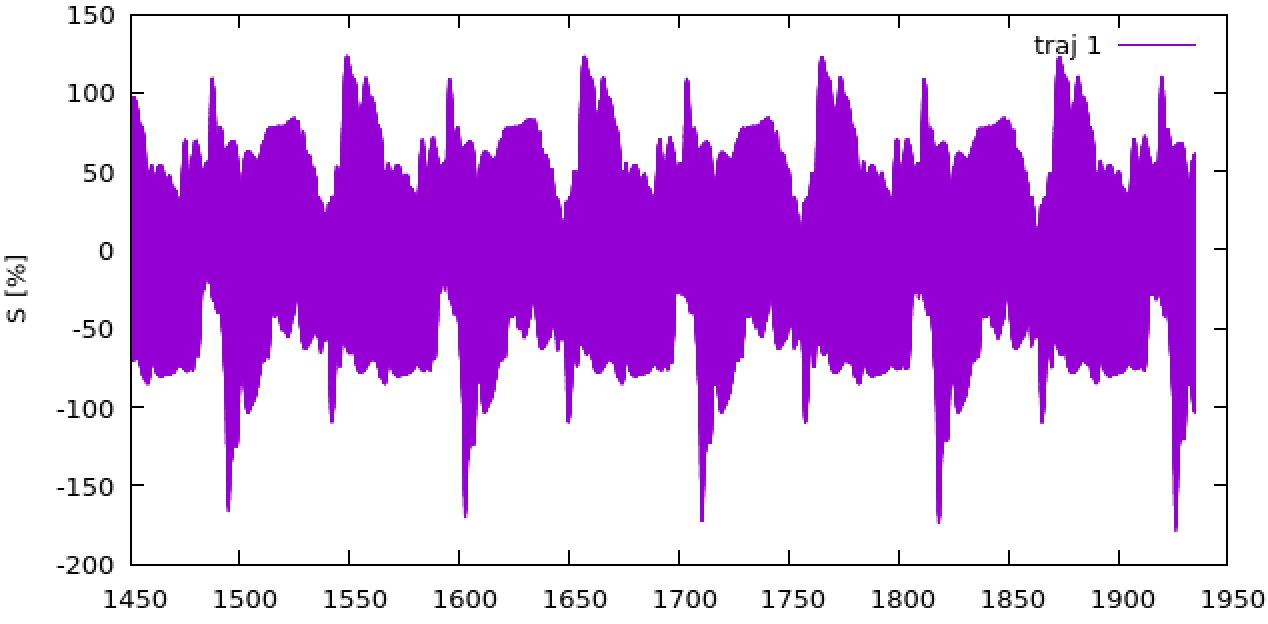
\includegraphics[angle=90,origin=c,width=0.35\textwidth]{figs/3_spin_selectivity_2.png}
	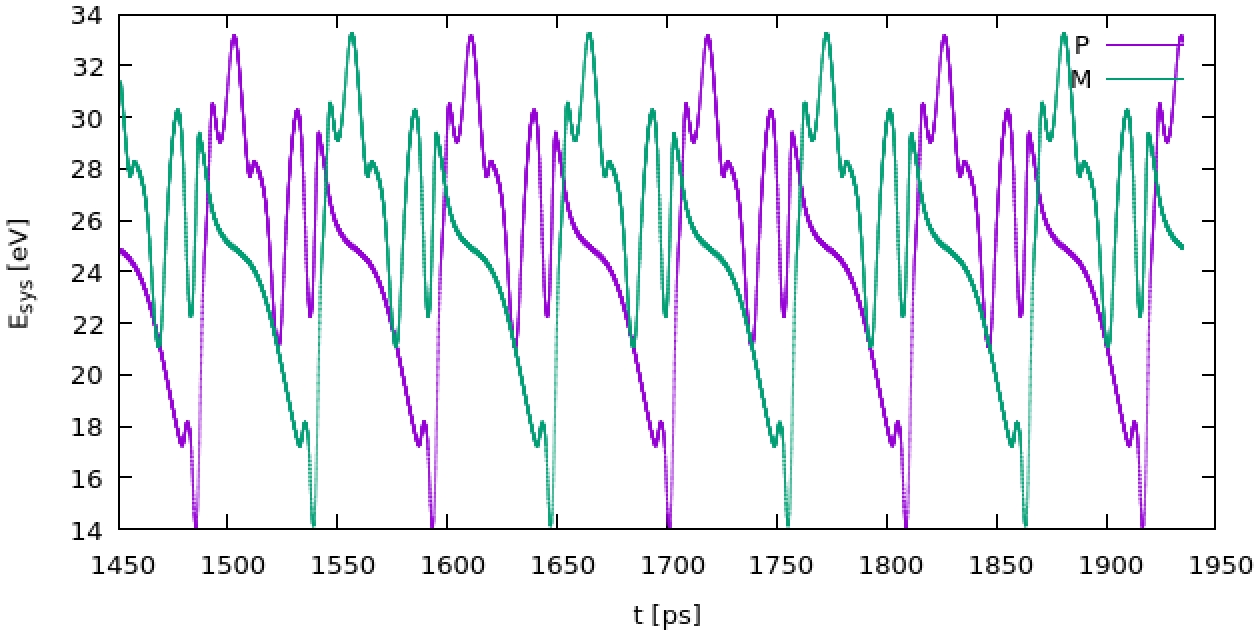
\includegraphics[angle=90,origin=c,width=0.35\textwidth]{figs/3_esys_2.png}
\end{figure}
\begin{figure}[!h]
\centering
	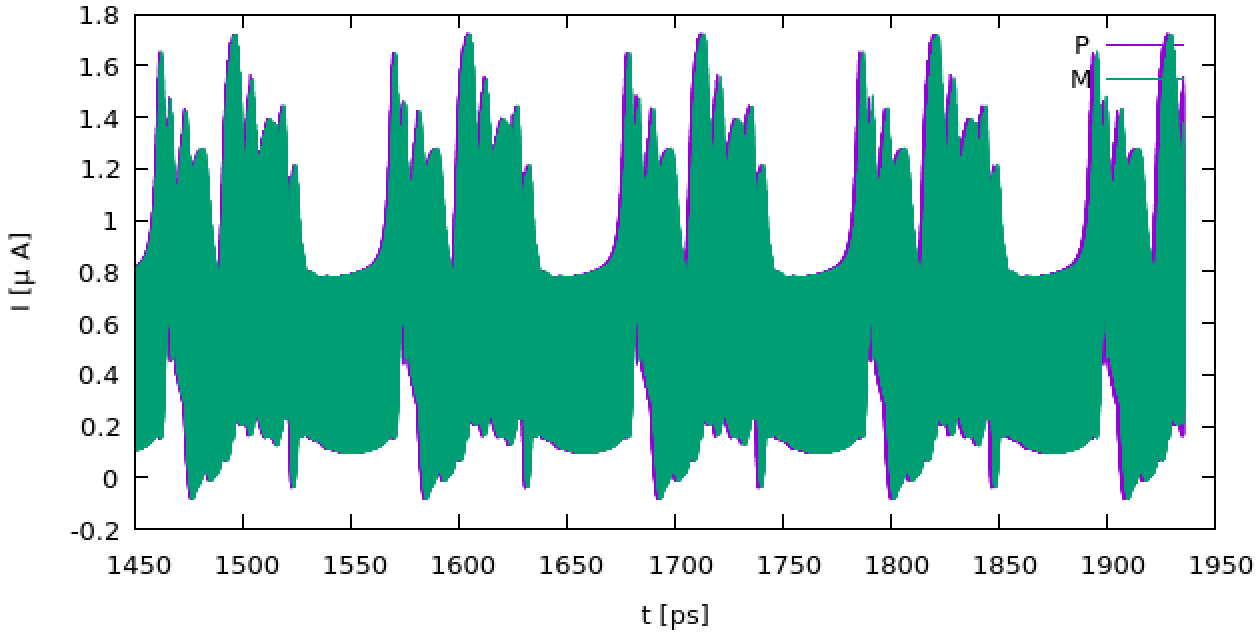
\includegraphics[width=0.7\textwidth]{figs/3_cur_3.png}
	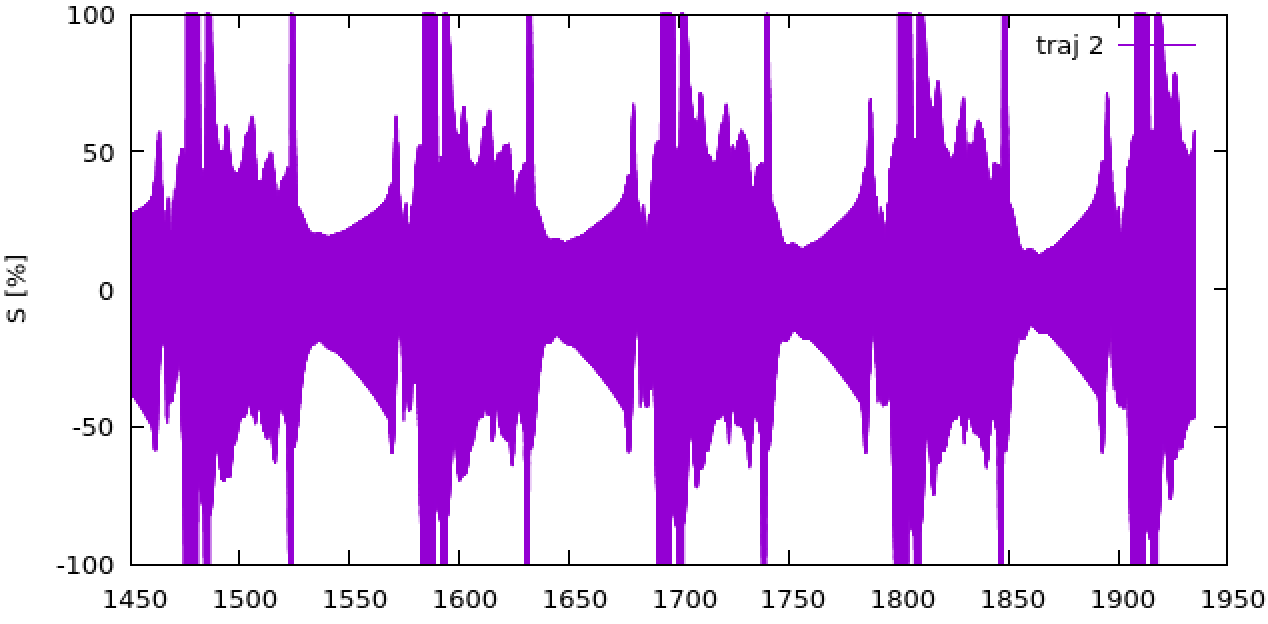
\includegraphics[width=0.7\textwidth]{figs/3_spin_selectivity_3.png}
	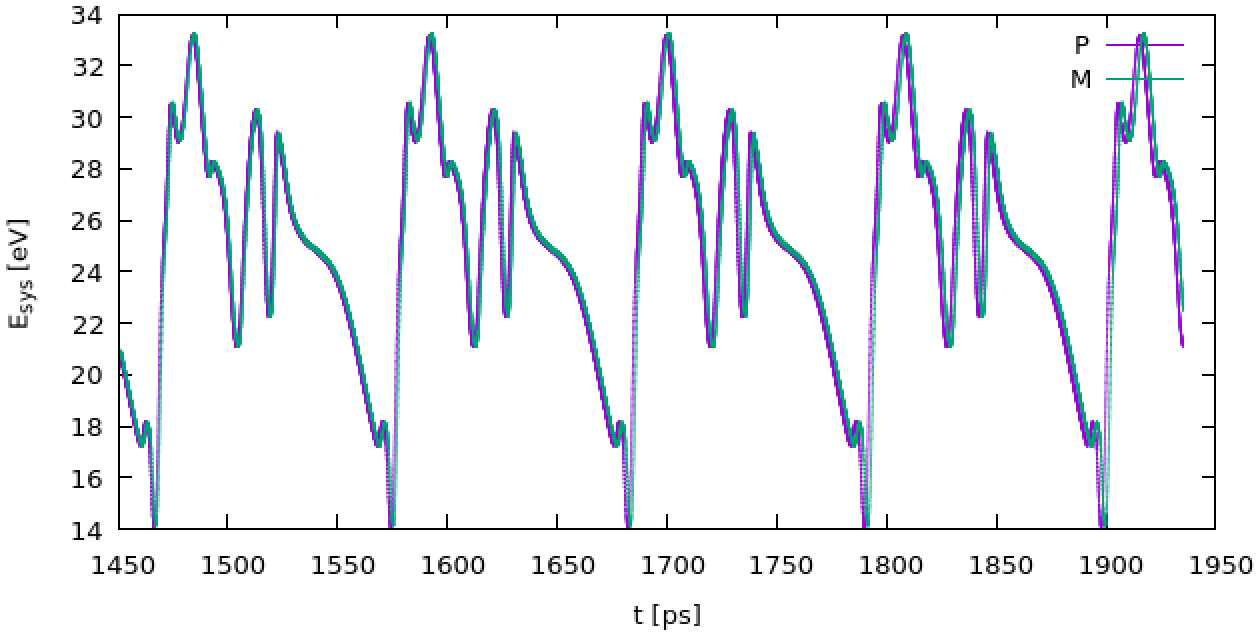
\includegraphics[width=0.7\textwidth]{figs/3_esys_3.png}
\end{figure}
\begin{figure}[!h]
\centering
	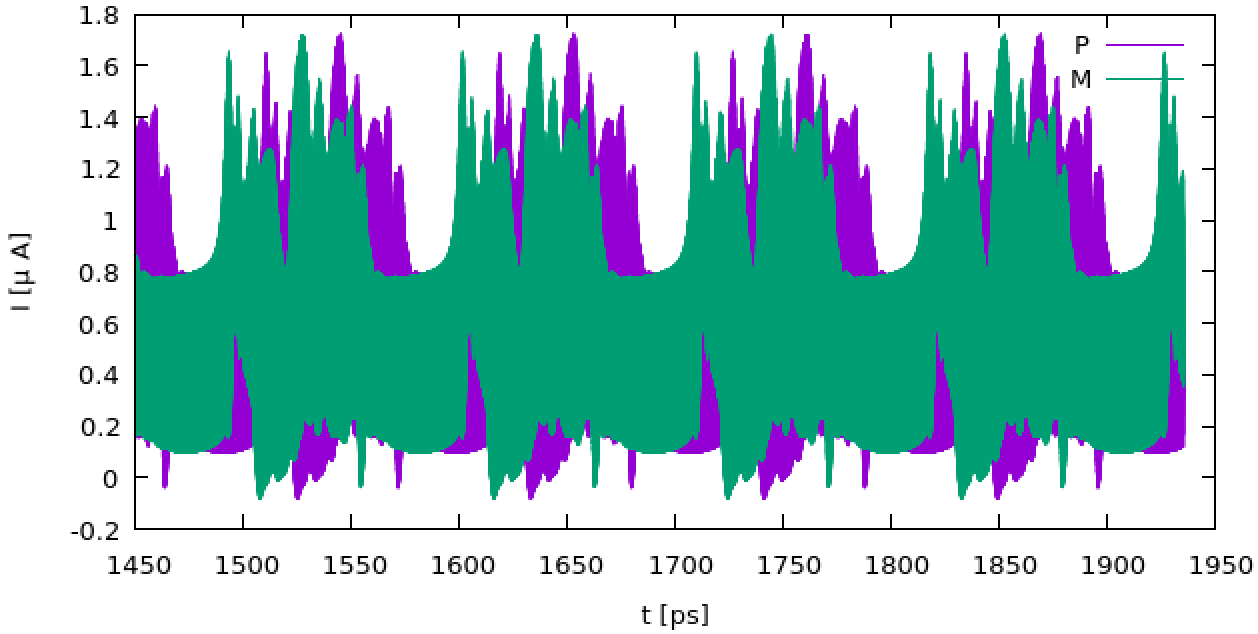
\includegraphics[width=0.7\textwidth]{figs/3_cur_4.png}
	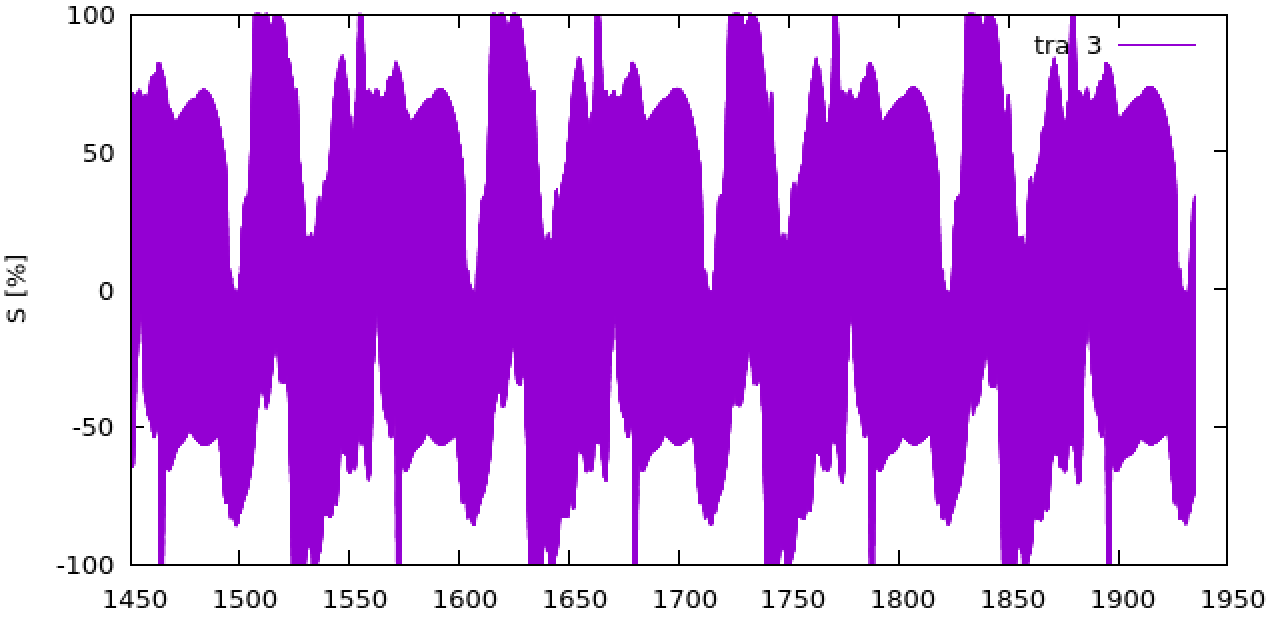
\includegraphics[width=0.7\textwidth]{figs/3_spin_selectivity_4.png}
	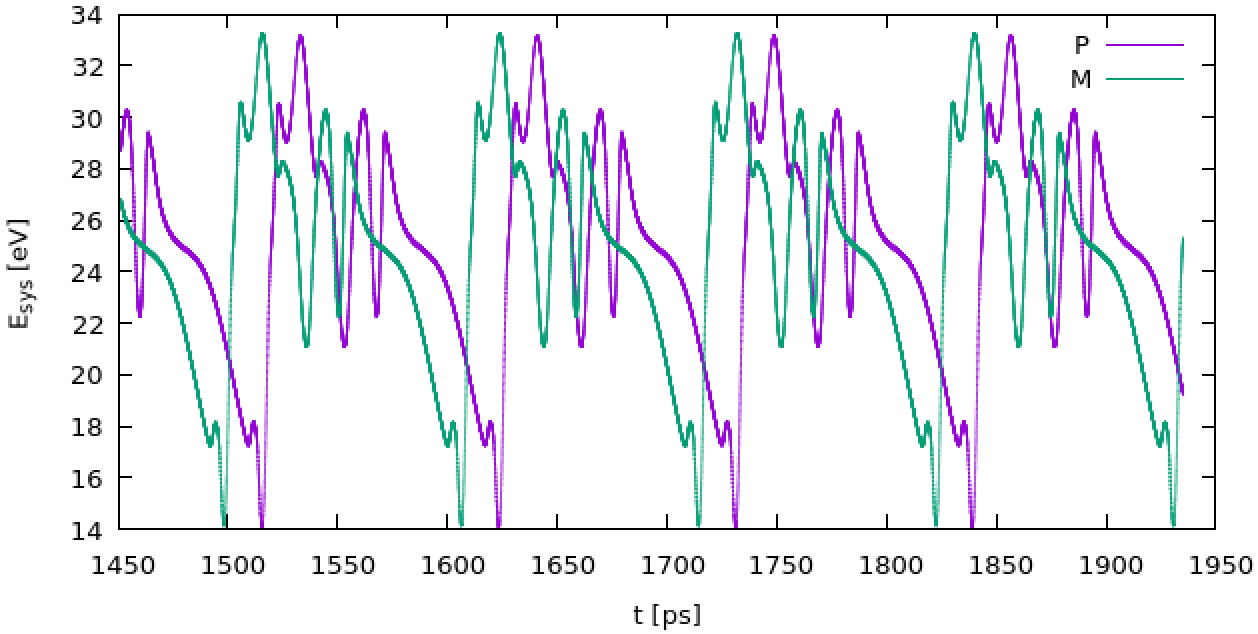
\includegraphics[width=0.7\textwidth]{figs/3_esys_4.png}
\end{figure}
\begin{figure}[!h]
\centering
	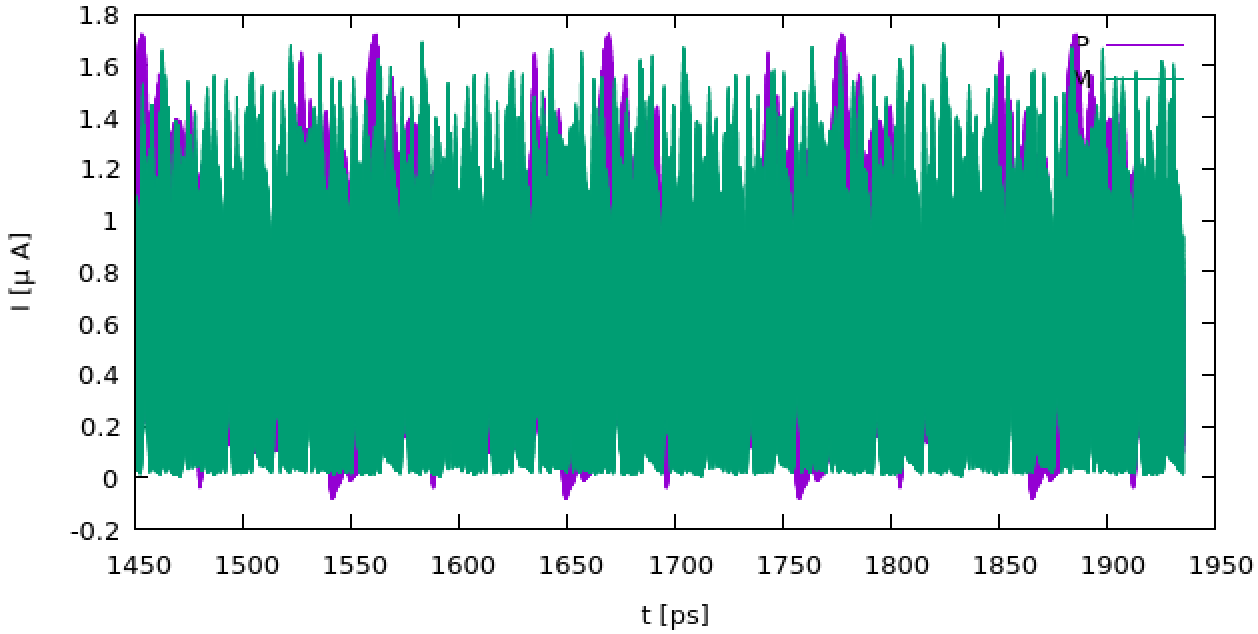
\includegraphics[angle=90,origin=c,width=0.35\textwidth]{figs/3_cur_5.png}
	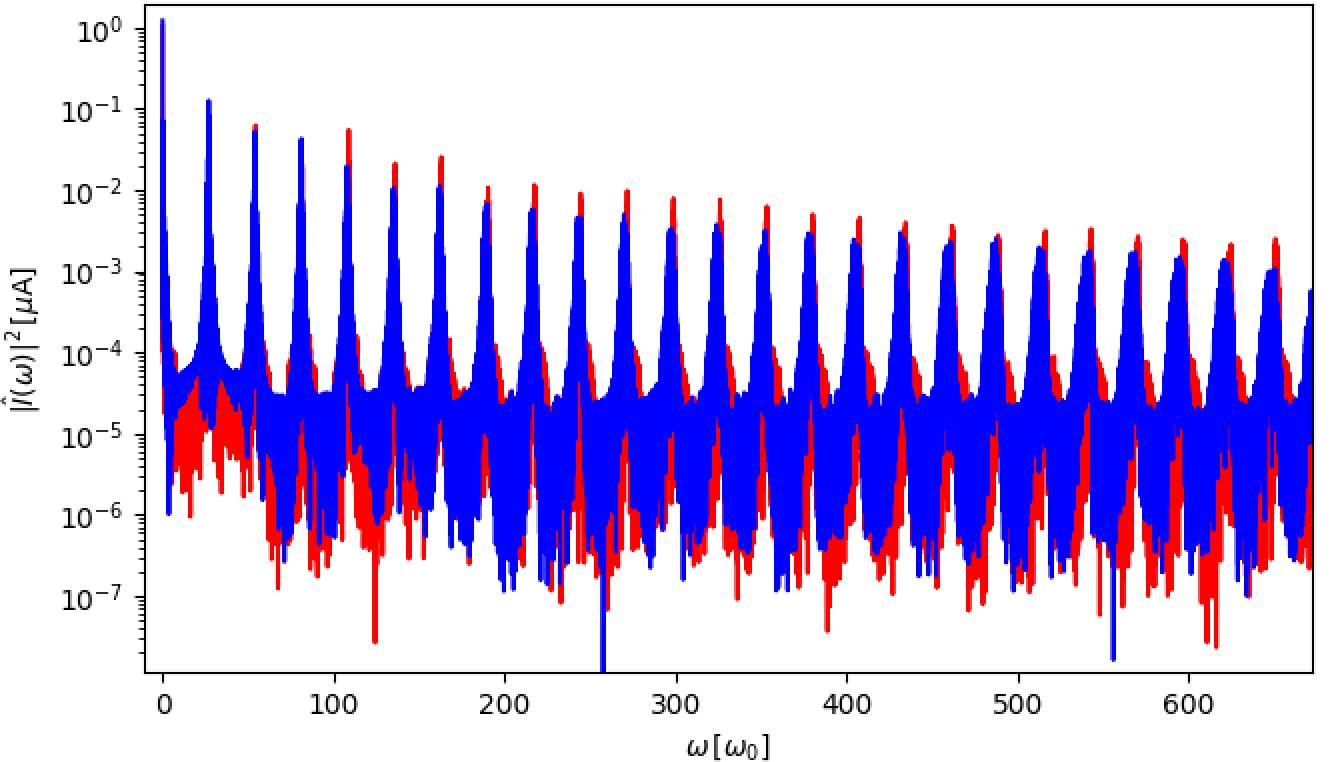
\includegraphics[angle=90,origin=c,width=0.35\textwidth]{figs/3_ft_5.png}
	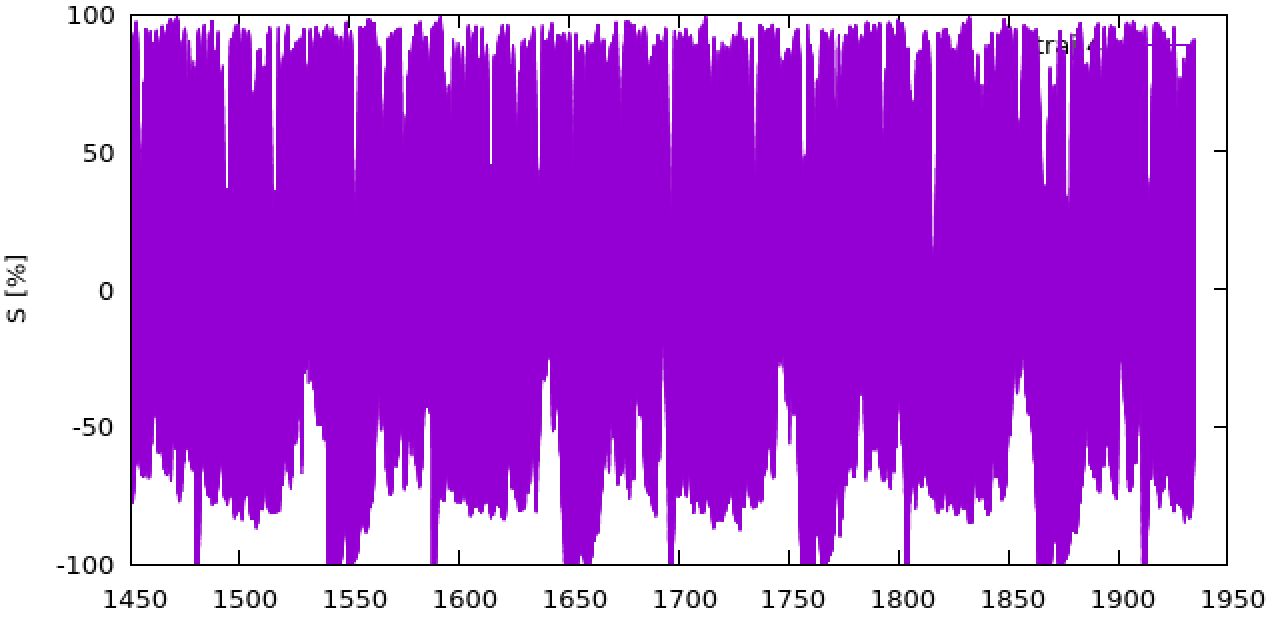
\includegraphics[angle=90,origin=c,width=0.35\textwidth]{figs/3_spin_selectivity_5.png}
	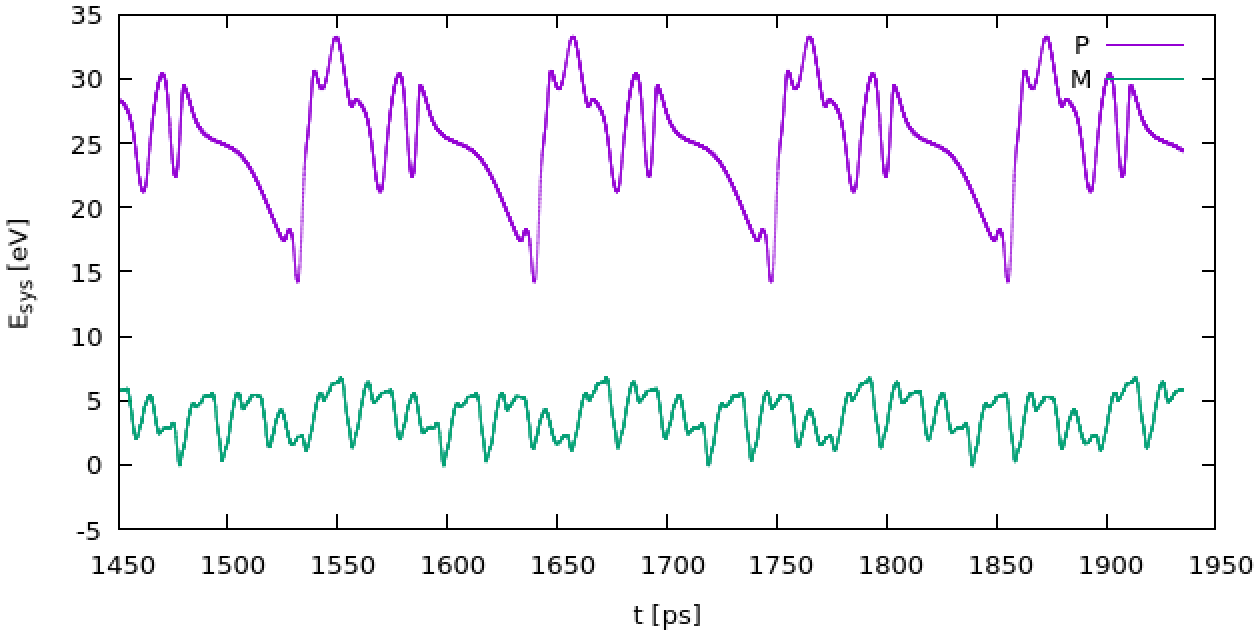
\includegraphics[angle=90,origin=c,width=0.35\textwidth]{figs/3_esys_5.png}
\end{figure}
\begin{figure}[!h]
\centering
	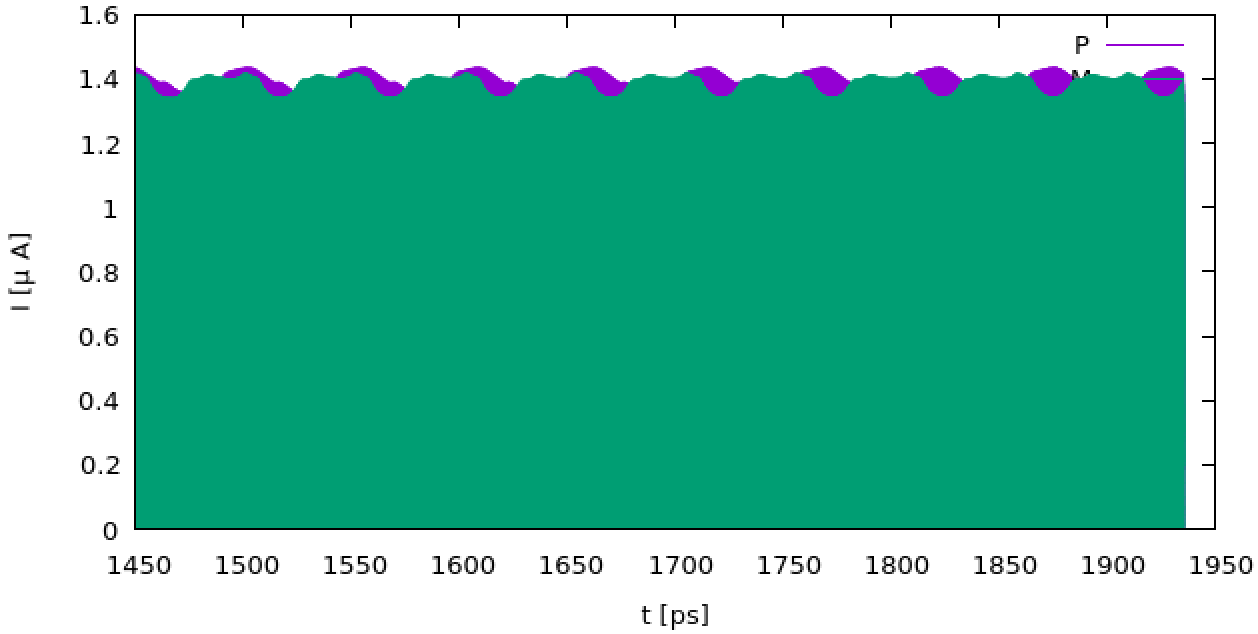
\includegraphics[width=0.7\textwidth]{figs/3_cur_6.png}
	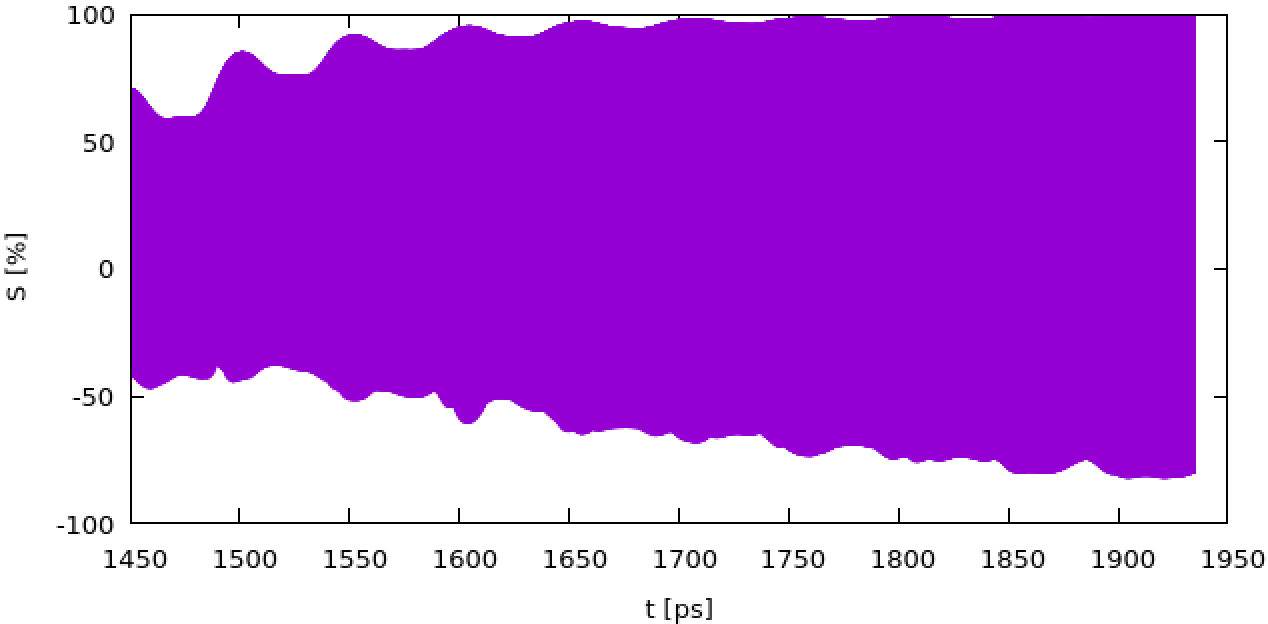
\includegraphics[width=0.7\textwidth]{figs/3_spin_selectivity_6.png}
	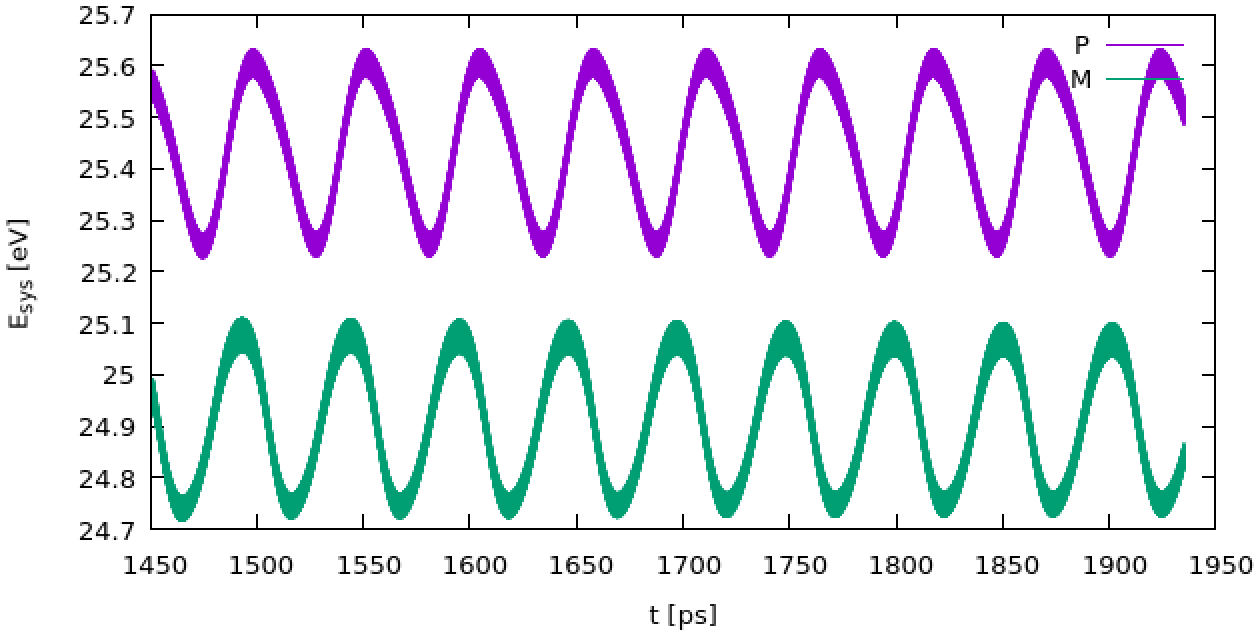
\includegraphics[width=0.7\textwidth]{figs/3_esys_6.png}
\end{figure}

\end{document}


